\documentclass[a4paper, 11pt]{article}

\usepackage[version=3]{mhchem}
\usepackage{siunitx}
\usepackage{graphicx}
\usepackage{amsmath}
\usepackage[total={16cm,25cm}, top=3cm, left=2.5cm, includefoot]{geometry}
\usepackage{pgfplots}
\usepackage{float}
\usepackage{amsfonts}
\usepackage{booktabs}
\usepackage{easytable}
\usepackage{mathtools}
\usepackage{comment}
\usepackage[makeroom]{cancel}
\renewcommand{\figurename}{Obrázek}
\renewcommand{\refname}{Zdroje}
\renewcommand{\tablename}{Tabulka}
\renewcommand{\contentsname}{Obsah}

\setlength\parindent{0pt}
\setcounter{section}{0}
\renewcommand{\labelenumi}{\alph{enumi}.}
\usepackage{xcolor}
\definecolor{light-gray}{gray}{0.95}
\newcommand{\code}[1]{\colorbox{light-gray}{\texttt{#1}}}
\newcommand{\logoCVUT}{
\includegraphics[width = 0.5\textwidth]{img/symbol_cvut_konturova_verze_cb.pdf}}
\newcommand{\logoFJFI}{
\includegraphics[width = 0.4\textwidth]{img/fjfi_logo.png}}

\begin{document}
% \section*{Seznam použitých veličin}
\addcontentsline{toc}{section}{Seznam použitých veličin}
\markboth{Seznam použitých veličin}{Seznam použitých veličin}

\renewcommand{\arraystretch}{1.2}
\begin{table}[H]
\begin{tabular}{p{1cm}l}
  $B_g$           & geometrický faktor (1/cm) \\
  $B_m$           & materiálový faktor (1/cm) \\
  $B_n$           & vlastní číslo (1/cm) \\
  $D$             & difúzní koeficient (cm) \\
  $\Phi$          & hustota toku neutronů (1/cm$^2$s) \\
  $k_{\text{ef}}$ & koeficient násobení (-) \\
  $k_{\infty}$    & koeficient násobení pro nekonečný systém (-) \\
  $\ell$          & střední doba života neutronů (s) \\
  $L$             & difúzní délka (cm) \\
  $L^2$           & difúzní plocha (cm$^2$) \\
  $\Lambda$       & střední doba vzniku neutronů (s) \\
  $n$             & hustota neutronů (1/cm$^3$) \\
  $N$             & počet neutronů (-) \\
  $P$             & výkon (tepelný) (W) \\
  $\Psi_n$        & vlastní funkce (-) \\
  $Q$             & zdroj neutronů (1/cm$^3$s) \\
  $\textbf{r}$    & polohový vektor (cm) \\
  $\rho$          & reaktivita (-) \\
  $\Sigma$        & makroskopický účinný průřez (1/cm) \\
  $\Sigma_a$      & makroskopický účinný průřez pro absorbci (1/cm) \\
  $\Sigma_f$      & makroskopický účinný průřez pro štěpení (1/cm) \\
  $t$             & čas (s) \\
  $T_e$           & perioda reaktoru (s) \\
  $v$             & rychlost (m/s) \\

\end{tabular}
\end{table}
\renewcommand{\arraystretch}{1}

% \section*{Seznam použitých zkratek}
\addcontentsline{toc}{section}{Seznam použitých zkratek}
\markboth{Seznam použitých zkratek}{Seznam použitých zkratek}

\renewcommand{\arraystretch}{1.2}
\begin{table}[H]
\begin{tabular}{p{1cm}l}
  AZ           & aktivní zóna \\
  1G           & 1-grupová \\
  2G           & 2-grupová \\
  FR           & rychlý reaktor -- Fast Reactor \\
  LS           & levá strana \\
  LT           & Laplaceova transformace \\
  LWR          & lehkovodní reaktor -- Light Water Reactor \\
  PS           & pravá strana \\
  ZV           & zpětná vazba \\
\end{tabular}
\end{table}
\renewcommand{\arraystretch}{1}


% titulní strana
\thispagestyle{empty}

\begin{center}
	{\LARGE
		České vysoké učení technické v Praze \par
		Fakulta jaderná a fyzikálně inženýrská
	}
    \vspace{10mm}

    \begin{tabular}{c}
		\textbf{Katedra jaderných reaktorů} \\[3pt]
    \end{tabular}

   \vspace{10mm} \logoCVUT \vspace{15mm}

   {\huge \textbf{Fyzika jaderných reaktorů}\par}
   \vspace{5mm}
   {\huge \textbf{Magisterské studium}\par}

   \vspace{15mm}
   {\Large \MakeUppercase{Státnicové otázky}}

   \vfill
   {\large
    \begin{tabular}{ll}
    Rok: & 2024
    \end{tabular}
   }
\end{center}

% Prohlášení
\newpage
\thispagestyle{empty}

%~
\vfill

\vspace{1em}
Čau ahoj. Právě čtete soubor magisterských státnicových otázek k předmětu Fyzika jaderných reaktorů, který byl vypracován za dlouhých zimních večerů v pokojíku ve Švýcarsku. Jedná se o sepis všech prezentací, skript a materiálů, ze kterých jsme během výuky čerpali, a které jsou dle mého názoru k pochopění nejdůležitější. Šlo zejména o:

\begin{itemize}
    \item prezentace k předmětu FARE (J. Frýbort),
    \item prezentace k předmětu DERF (J. Frýbort a P. Suk),
    \item přednášky z předmětu SMRF (O. Huml),
    \item přednášky z předmětu KID (O. Huml),
    \item zápisky z předmětu KID (O. Huml),
    \item Dynamika jaderných reaktorů -- B. Heřmanský,
    \item Nuclear Reactor Physics -- W. Stacey,
    \item Introduction to Nuclear Engineering -- J. Lamarsch,
    \item manuál ke kódu NJOY,
    \item manuál ke kódu SCALE,
    \item manuál ke kódu MCNP,
    \item prezentace MCNP z LANL,
    \item apod.
\end{itemize}

Pokud najdete chybu, hoďte issue na Git: \\

\rm Hodně zdaru!

\vspace{2em}

\clearpage{\pagestyle{empty}}

\include{none}

\newpage
\parskip=0pt
\begin{small}
\tableofcontents
\end{small}
\parskip=7pt
\newpage

\section[Difúzní teorie]{Odvození a využití difuzní teorie v reaktorové fyzice}
\section{Jaderná data v reaktorové fyzice}

Jadrná data jsou prostředek, díky kterému matematický popis systému dostává skutečný fyzikální význam. Každé řešení difúzní či transportní rovnice je tak přesné, jak přesné jsou právě jaderná data. Obecně jsou 2 způsoby, jak data získat:

\begin{itemize}
  \item Teoretické určení -- je možné určit průřezy pro různé energetické oblasti (pružný rozptyl), či popsat izolovanou rezonanci (Breit-Wignerova formule), nicméně není možné je aplikovat obecně (neexistuje přesný matematický popis štěpení, komplikace v rezonanční oblasti apod.).
  \item Experimentální určení -- důležitější a významnější způsob určování dat, nicméně takovéto hodnoty mají pouze omezenou a konečnou přesnost.
\end{itemize}

Dále je důležité si klást otázku, k čemu data potřebujeme. Pro reaktorovou fyziku stačí energetické rozmezí 10 $\mu$eV až 20 MeV (knihovny ENDF/B, JEFF, atd.), jiné je to ale např. pro astrofyziku, částicovou fyziku atd.\\

Mezi jaderná data je možné řadit: mikroskopické účinné průřezy, diferenciální průřezy (úhlově i energeticky), rozpadové konstanty, výtěžky ze štěpení, spektra ze štěpení apod.\\

Dále existují 2 přístupy:

\begin{itemize}
  \item spojitá data (stochastické výpočty),
  \item grupová data (deterministické výpočty).
\end{itemize}

\subsection{Proces zaznamenávání jaderných dat}

\subsubsection{Příprava a shromažďování}

Veškeré experimentální výsledky jsou shromažďovány v mezinárodní databází \textbf{EXFOR} podle standardu z konference v Moskvě roku 1969. Současně obsahuje přibližně 23 tisíc sad experimentálních měření. 

\subsubsection{Evaluace (zhodnocení) a ukládání}

Následuje evaluace (zhodnocení) v jednom ze světových datových center (USA, Evropa, Jaoponsko, Rusko, Čína). Proces evaluace má za úkol data protřídit, něco vyházet, něco zkombinovat (hlavně v oblasti rezonancí, používá se metoda nejmenších čtverců, Breit-Wigner apod.). Využívají se k tomu specializované kódy, např. \textbf{GNASH}, \textbf{EMPIRE}, \textbf{SAMMY}, jejichž aplikace je závislá na energetické rozsahu. Důraz se klade na aktinoidy a štěpení.\\

Takto zhodnocená data se ukládají v tabulce ve formátu \textbf{ENDF-6} (standard z roku 1968, ale za mě je nepřehledný a dost naprd), který je čitelný jazykem FORTRAN.V budoucnu se snad  nahradí modernějším a obecnějším formátem \textit{Generalized Nuclear Data}, který umí XML a JSON.

\subsubsection{Verifikace}

Jde pouze o kontrolu, jestli jsou zhodnocená data správná, dodržují fyziku a chovají se tak, jak se očekává.

\subsubsection{Validace}

Aby bylo možné data použít, je potřeba je ověřit s experimenty, tzv. validovat. To probíhá pomocí benchmarků, kde se srovnává $k_\text{ef}$, kinetické parametry či vyhořívání paliva. K validaci slouží mezinárodní projekt \textbf{ICSBEF} (International Criticality Safety Benchmark Evaluation Project) obsahující srovnávací úlohy pro kritické konfigurace a pro stínění. Dále může posloužit databáze \textbf{SFCOMPO-2.0}, která obsahuje data o složení palivových vzorků pro různé druhy reaktorů.\\

Tímto způsobem vznikají zvalidované jaderné knihovny, které si kdokoliv může stáhnout a použít. Existuje několik knihoven, v reaktorové fyzice se používají zejména:

\begin{itemize}
  \item ENDF/B -- původ USA (Brookhaven),
  \item JEFF -- původ Evropa,
  \item JENDL -- původ Japonsko,
  \item CENDL -- původ Čína.
\end{itemize}

Každá knihovna se pak hodí pro něco jiného, např. JEFF se hodí pro rychlé sodíkové reaktory, protože lépe zachycuje reakce se sodíkem. Ale asi záleží na osobním vkusu.

\subsection{Proces zpracování jaderných dat}

V následném zpracování je rozhodující, jestli nás zajímá spojitá či grupová struktura. V každém případě se k následujícímu popisu hodí např. kód \textbf{NJOY} (s jiným kódem jsme nepracovali, tudíž nic jiného neznám).\\

Ten funguje na principu jednotlivých modulů, které mezi sebou komunikují. Záleží na uživateli, co od dat požaduje. Dále jsou vyčteny ty nejdůležitější procedury, nicméně je jich celá řada dalších (moduly \textbf{GASPR} -- zahrnuje reakce produkující plyny (helium, vodík...), \textbf{HEATR} -- posuzuje radiační ohřev a radiační poškození, \textbf{PURR} -- příprava nerozlišených rezonancí pro stochastické kódy, či \textbf{THERMR} -- analýza rozptylu tepelných neutronů; které sem v životě nepoužil).\\

\subsubsection{Linearizace}

Získaná a zhodnocená data jsou bodová. Pro získání informací mimo body se používá interpolace (prvním krokem je vždy lineární interpolace) případně matematický popis pro rezonance. V dalším kroku následují nelineární interpolace, které se ověřují zpětným součtem totálního průřezu $\rightarrow$ iterativní proces.\\

NJOY nejprve vezme ENDF formát a přetvoří ho do PENDF formátu (Pointwise ENDF), se kterým dále pracuje. O to se stará modul \textbf{RECONR}, který umí zrekonstruovat rezonance a nelineární aproximace z ENDF. Opět probíhá kontrola přes součet totálního průřezu.

\subsubsection{Úprava na teplotu}

Zhodnocená jaderná data se ukládají pro teplotu 0~K. Nicméně díky Dopplerově efektu (rozšiřování rezonancí) je důležité data přepočíst na požadovanou teplotu (jde zejména o rezonanční a tepelnou oblast), čímž se mění energetická síť.\\

V NJOY provádí modul \textbf{BROADR}. Ten to provádí pomocí přesného řešení efektivního účinného průřezu (to je ten, který se ve FARE zaváděl pro popis Dopplerova efektu). Je definován tak, aby dával pro nuklidy v klidu stejnou reakční rychlost jako pro nuklidy v pohybu. Obecně klesá vrchol rezonancí na úkor šířky tak, aby plocha pod rezonancí zůstávala konstantní. Oblast 1/v je v pořádku, rovněž oblast nad 100~keV, nad kterou jsou rezonance nerozlišené

\subsubsection{Grupování}

Pro deterministické kódy je důležité data energeticky zgrupovat. Tento proces požaduje zachování reakční rychlosti. V podstatě jde o vážený průměr přes hustotu toku neutronů, díky čemuž je hustota toku nepřímo úměrná celkovému makroskopickému průřezu, viz:

\begin{equation}
  \boxed{
    \bar{\sigma_g} = \dfrac{\int_g \sigma(E) \Phi(E) \text{d}E}{\int_g \Phi(E) \text{d}E}.}
    \label{grupovani}
\end{equation}

V závislosti na analyzovaném systému se musí vhodně odhadnout spektrum neutronů, neboli jakou vážící funkci použiji.\\

Také se musí zvolit vhodná grupová struktura zohledňující očekávané spektrum v systému. Příliš jemná struktura zvyšuje výpočetní náročnost, naopak příliš hrubá zkresluje výsledky (může přehlédnout potřebné rezonance, překryv rezonancí FPs, aktinoidů či okolního materiálu apod.). Obecně rychlé systémy vyžadují více (tisíce) grup, než tepelné systémy. Např. moji oblíbení zástupci jsou XMAS pro tepelný reaktor a Vitamin-j pro rychlý reaktor, což jsou podmnožiny velké grupové struktury zavedené v ERANOSu, které se nějak dochovaly a používají se stále.\\

V NJOY grupování provádí modul \textbf{GROUPR}, čímž vznikne formát GENDF (Groupwise ENDF). Ten dále připravuje matice přechodu mezi grupami (rozptylové přechody).

\subsubsection{Zohlednění samostínění}

Grupování průřezů musí rovněž zohledňovat vliv samostínění. S rostoucí hodnotou účinného průřezu se snižuje střední volná dráha neutronů (roste $\Sigma$, logicky z definice klesá $\lambda$), čímž klesá hustota toku (to je ten důvod, proč se projevuje samostínění v palivu. Na periferii peletky dochází k poklesu hustoty toku, proto střed vyhořívá pomaleji). V praxi se tento efekt projevuje v rezonancích, kde dochází právě k nárůstu průřezu, a tudíž k poklesu hustoty toku. Z toho tedy platí jednoduchá relace:

\begin{equation}
  \boxed{
    \Phi(E) \sim \dfrac{1}{\Sigma_t(E)},}
    \label{samostineni}
\end{equation}

\noindent (znamená to, že když se např. vykreslí hustota toku v palivu, tak dochází k prudkým poklesům v oblastech rezonance. I proto je dobré volit vhodnou grupovou strukturu, abychom tento efekt zaznamenali).\\

Pokud bychom chtěli dle rovnice \eqref{grupovani} data grupovat, je potřeba znát hustotu toku, což neznáme, protože je ovlivněna právě samostníněním. Pomocí přepisu \eqref{samostineni} do \eqref{grupovani} se pro vybraný nuklid $i$ rovnice přepíše do tvaru:

$$ \bar{\sigma}_g^i = \dfrac{\int_g \dfrac{\sigma^i(E)}{\Sigma_t(E)} \text{d}E}{\int_g \dfrac{1}{\Sigma_t(E)} \text{d}E} = \dfrac{\int_g \dfrac{\sigma^i(E)}{N^i \sigma_t^i(E) + \sum_j N^j \sigma_t^j(E)} \text{d}E}{\int_g \dfrac{1}{N^i \sigma_t^i(E) + \sum_j N^j \sigma_t^j(E)} \text{d}E} = \dfrac{\int_g \dfrac{\sigma^i(E)}{\sigma_t^i(E) + \sigma_0^i(E)} \text{d}E}{\int_g \dfrac{1}{\sigma_t^i(E) + \sigma_0^i(E)} \text{d}E},$$

\noindent kde $\sigma_0^i(E) = \sum_j \dfrac{N^j}{N^i} \sigma_t^j(E).$\\

Postupuje se pomocí tzv. \textbf{Bondarenkovy metody}, která zanedbává některé jemné efekty tím, že zavede efektivní hodnotu $\bar{\sigma}_0^i$ středovanou přes energii grupy:

$$ \bar{\sigma}_0^i = \dfrac{\int_g \sigma^i_0(E) \text{d}E}{\int_g \text{d}E}.$$

Dále se používají tzv. \textbf{Bondarenkovy faktory} $F_g^i(\bar{\sigma}_0^i, T)$, který určují poměr mezi konkrétním grupovým průřezem $\bar{\sigma}_g^i(\bar{\sigma}_0^i, T)$ (ten který hledáme, tedy reakce na $i$-tém nuklidu v sumě okolí přes $j$) a efektivním průřezem, který by platil v nekonečně zředěném prostředí $\bar{\sigma}_g^{i,\infty}$ (jde o největší možný, tedy pokud by tam ten okolní samostínící materiál $j$ nebyl a $\bar{\sigma_0^i} \rightarrow \infty$):

$$ \bar{\sigma}_g^{i,\infty} = \dfrac{\int_g \dfrac{\sigma^i(E)}{\sigma_t^i(E) + \bar{\sigma}_0^i} \text{d}E}{\int_g \dfrac{1}{\sigma_t^i(E) + \bar{\sigma}_0^i} \text{d}E} = |\bar{\sigma_0^i} \rightarrow \infty| = \dfrac{\int_g \sigma^i(E) \text{d}E}{\int_g \text{d}E},$$
$$ F_g^i (\bar{\sigma_0^i}, T) = \dfrac{\bar{\sigma}_g^i(\bar{\sigma}_0^i, T)}{\bar{\sigma}_g^{i,\infty}}. $$

V praxi jsou napočteny různé hodnoty Bondarenkových faktorů pro odlišné $\bar{\sigma}_0^i$ a teploty (ty jsou uloženy v logaritmických rozestupech a dá se mezi nimi interpolovat), nekonečné zředění $\bar{\sigma}_g^{i,\infty}$ není těžké spočíst, jelikož se nestředuje přes hustotu toku, tudíž výsledné určení grupového průřezu se stanoví:

\begin{equation}
  \boxed{
    \bar{\sigma}_g^i(\bar{\sigma}_0^i, T) = \bar{\sigma}_g^{i,\infty} \cdot F_g^i (\bar{\sigma}_0^i, T).}
\end{equation}

Ve zkratce: pokud grupový průřez pro daný nuklid  $i$ převyšuje průřez skutečného okolí $j$ (rezonance), dochází k efektu samostínění a reakční rychlost klesá, což se vyjádří poklesem grupového průřezu, což má na svědomí právě Bondarenkův faktor.\\

I tento proces má na svědomí modul \textbf{GROUPR}. Použije se tradiční váhová funkce hustoty toku neutronů (Maxwell, 1/v apod.), která má ale reálně propady, k čemuž se aproximuje pomocí rozkladu do Legendrových polynomů $\Phi_l(E)$:

$$\Phi_l(E) = \dfrac{C(E)}{\left [ \sigma_t^i(E) + \bar{\sigma}_0^i \right ]^{l+1}},$$

\noindent kde $C(E)$ představuje váhovou funkci.

\subsubsection{Spojování}

Pokud nás nezajímá grupová struktura ale spojitá knihovna pro stochastické kódy, je možné hodnoty exportovat pomocí modulu \textbf{ACER}. Ten využívá lineární aproximace a vytváří ACE knihovnu (A Compact ENDF), která může být vyexportována do formátu XSDIR vhodné např. pro \textbf{Serpent}.
\section[Transportní rovnice]{Odvození a využití transportní teorie v reaktorové fyzice}

Transportní rovnice je základní matematický model používaný v reaktorové fyzice k popisu pohybu a interakce neutronů v materiálu. Její cílem je určit rozložení neutronů v prostoru, energii a čase v jaderném reaktoru nebo jiném prostředí.

Momentálně se jedná o rovnici, která co nejvěrněji popisuje chování a šíření neutronů, nicméně její zápis je příliš složitý a neexistuje obecné analytické řešení. Z toho důvodu je nutné přecháet k určitým zjednodušením, kterými může být například difúzní rovnice.

\subsection{Boltzmanova integro-diferenciální transportní rovnice}

Odvození musí nutně vycházet z dějů, které má popisovat. Vzhledem k běžným podmínkám v reaktorech je možné popis chování neutronů zúžit na úlohu neutrálních částic pohybujících se podle zákonitostí klasické mechaniky s kvantovým popisem jejich interakcí s jádry okolního prostředí.

Cílem je převést izolovanou částicovou povahu interakcí neutronů na spojitou veličinu.

\subsubsection{Předpoklady}

Pro odvození musíme předpokládat:

\begin{itemize}
  \item dostatečná populace neutronů, abychom mohli uvažovat statistické středování,
  \item neutrony interagují pouze s jádry okolí (která jsou v klidu) a nikoliv mezi sebou $\rightarrow$ v reaktorech splněno vždy (projevuje se až pro $\Phi > 10^{20}$ 1/cm$^2$/s).
\end{itemize}

\subsubsection{Matematický aparát}

Pro odvození je potřeba zavést:

\textbf{a) Nezávislé proměnné}:

Nezávislé proměnné představují souřadnice, pomocí kterých jsme schopni neutronům přiřadit bod fázového prostoru. Pro jednoznačné určení je potřeba 6~nezávislých proměnných (v klasické mechanice jde o 3~složky polohového vektoru a 3~složky vektoru rychlosti), nicméně v tomto případě se od vektoru rychlosti přechází ke směru pohybu a velikosti rychlosti.

Pro popis tedy předpokládáme:

\begin{itemize}
  \item polohový vektor $\textbf{r} = (x, y, z)$ -- 3 složky,
  \item směrový vektor $\Omega = (\phi, \theta)$ -- 2 složky,
  \item (kinetická) energie $E$ -- 1 složka.
\end{itemize}

Pro případný přepočet poté platí:

$$ v = \sqrt{\dfrac{2m}{E}}, $$
$$ \textbf{v} = v \Omega. $$

Časovou závislost zanedbáváme a na čas nahlížíme jako na parametr, nikoliv souřadnici.

\textbf{b) Fázový prostor:}

Představuje prostor pro popis neutronových interakcí. Základním předpokladem je zachování částicové povahy neutronů při využití statistické povahy pohybu velkého množství částic. Jednotlivé srážky se proto odehrávají ve statisticky středovaném \textbf{elementu fázového prostoru} $\Delta \textbf{P}$:

$$ \Delta \textbf{P} = \Delta \textbf{r} \Delta \Omega \Delta \textbf{E}. $$

Počet neutronů v $\Delta \textbf{P}$ se může změnit vlivem změny v dílčích parametrech, tedy:

\begin{itemize}
  \item v $\Delta \textbf{r}$ -- únikem z $\Delta \textbf{r}$, případně absorbcí nebo vznikem v $\Delta \textbf{r}$,
  \item v $\Delta \Omega$ -- rozptylem,
  \item v $\Delta E$ -- zpomalením, nebo zrychlením.
\end{itemize}

\textbf{c) Závislé proměnné:}

Dále je potřeba zavést závislé proměnné (závislé od toho, že jsou závislé na těch nezávislých a času), které představují sledované veličiny.

Sem řadíme 3 základní:

\begin{itemize}
  \item úhlová hustota neutronů $n(\textbf{r}, \Omega, E, t)$ (1/cm$^3$) -- skalár,
  \item úhlová hustota toku neutronů $\Omega(\textbf{r}, \Omega, E, t)$ (1/cm$^2$/s) -- skalár (ale bacha, neplést se směrovým vektorem $\Omega$),
  \item úhlová hustota proudu neutronů $\textbf{J}(\textbf{r}, \Omega, E, t)$ (1/cm$^2$/s) -- vektor
\end{itemize}

s definovanými vztahy:

\begin{equation}
  \boxed{
  \Phi(\textbf{r}, \Omega, E, t) = v \cdot n(\textbf{r}, \Omega, E, t),
  \label{definice_hustota_toku}}
\end{equation}

\begin{equation}
  \boxed{
  \textbf{J}(\textbf{r}, \Omega, E, t) = \Omega \cdot \Phi(\textbf{r}, \Omega, E, t).
  \label{definice_hustota_proudu}}
\end{equation}

Pro kontext, \textbf{$\Phi$ udává celkový součet drah všech neutronů za sekundu v jednotkovém objemu fázového prostoru}, zatímco \textbf{$\textbf{J}$ udává počet neutronů, který prochází na steradián, energii a plochu ve směru $\Omega$ plochou kolmou k $\Omega$ v čase}. Tedy, zatímco $n$ a $\Phi$ se vztahují k objemu, $\textbf{J}$ se vztahuje k ploše.

\subsubsection{Odvození}

Nejprve je potřeba si uvědomit, jak popisujeme interakce neutronů s jádry. Pravděpodobnost interakce je dána $\sigma$ (cm$^2$) a $\Sigma$ (1/cm), přičemž mezi možné interakce řadíme pouze: rozptyl, radiační záchyt a štěpení, případně absorbci (což je součet štěpení a radiačního záchytu).

\textbf{Makroskopický účinný průřez pro interakci $i$ na jádře $j$} -- $\Sigma_{ij}(\textbf{r}, E, t)$ definujeme jako podíl pravděpodobnosti interakce neutronu reakcí $i$ s jádrem $j$ na jednotku délky dráhy.

Dále \textbf{reakční rychlost pro interakci $i$ na jádře $j$} -- $F_{ij}(\textbf{r}, E, t)$ určíme jako:

$$ F_{ij}(\textbf{r}, E, t) = \Sigma_{ij}(\textbf{r}, E, t) \Phi(\textbf{r}, E, t). $$

Při předpokladu nezávislosti jednotlivých interakcí (abychom mohli průřezy sčítat) je možné definovat totální makroskopický účinný průřez:

$$ \Sigma_i(\textbf{r}, E, t) = \sum_{j=1}^J \Sigma_{ij}(\textbf{r}, E, t) = \sum_{j=1}^J N_j(\textbf{r}, t) \sigma_{ij}(E). $$

Dále si pro popis rozptylu zavedeme \textbf{diferenciální rozptylové jádro} -- $f_s(\Omega' \cdot \Omega, E' \rightarrow E)$ (-) tak, že:

\begin{itemize}
  \item $f_s(\Omega' \cdot \Omega, E' \rightarrow E) \Delta \Omega \Delta E$ značí poměrnou pravděpodobnost rozptylu ze směru $\Omega'$ a energie $E'$ do rozsahu směrů $\Delta \Omega$ a energií $\Delta E$,
  \item pro rozptyl na jádře $j$ platí:
\end{itemize}
$$\Sigma_{sj}(\textbf{r}, \Omega' \cdot \Omega, E' \rightarrow E, t) = \Sigma_{sj}(\textbf{r}, E', t) f_s(\Omega' \cdot \Omega, E' \rightarrow E), $$

\begin{itemize}
  \item pro účely normalizace platí:
\end{itemize}
$$\int_\mathbb{R^+} \int_{4 \pi} f_s(\Omega' \cdot \Omega, E' \rightarrow E) \text{d} \Omega \text{d}E = 1. $$


Pro odvození musíme vycházet z bilanční rovnice neutronů, kde sledujeme změnu počtu neutronů v libovolném elementu fázového prostoru tvořeném objemem $V$ a $\Delta \Omega \Delta E$ během časového intervalu $\Delta t$.

Jednodušeji řečeno posuzujeme jednotlivé příspěky či ztráty neutronů:

\begin{equation}
  \boxed{
  \begin{pmatrix} \text{počet neutronů} \\ \text{v čase } t + \Delta t \end{pmatrix} = \begin{pmatrix} \text{počet neutronů} \\ \text{v čase } t \end{pmatrix} + \begin{pmatrix} \text{zisk neutronů} \\ \text{během } \Delta t \end{pmatrix} - \begin{pmatrix} \text{ztráta neutronů} \\ \text{během } \Delta t \end{pmatrix}.
  \label{bilancni_rovnice}}
\end{equation}

Nyní popíšeme jednotlivé stavy:

\textbf{a) Počet neutronů v čase $t + \Delta t$:}

$$ \Delta \Omega \Delta E \int_V n(\textbf{r}, \Omega, E, t + \Delta t) \text{d}V $$

\textbf{b) Počet neutronů v čase $t$:}

$$ \Delta \Omega \Delta E \int_V n(\textbf{r}, \Omega, E, t) \text{d}V $$

\textbf{c) Zisk neutronů během $\Delta t$:}

Zisk neutronů se skládá ze zisku:

\begin{itemize}
  \item rozptylem:
\end{itemize}
$$ \Delta \Omega \Delta E \Delta t \int_V \int_\mathbb{R^+} \int_{4 \pi} f_s(\Omega' \cdot \Omega, E' \rightarrow E) \Sigma_s(\textbf{r}, E', t) \Phi(\textbf{r}, \Omega', E', t) \text{d}\Omega' \text{d}E' \text{d}V, $$

\begin{itemize}
  \item štěpením:
\end{itemize}
$$ \Delta \Omega \Delta E \Delta t \dfrac{\chi(E)}{4 \pi} \int_V \int_\mathbb{R^+} \int_{4 \pi} \nu(E') \Sigma_f(\textbf{r}, E', t) \Phi(\textbf{r}, \Omega', E', t) \text{d}\Omega' \text{d}E' \text{d}V. $$


Štěpení se předpokládá izotropní (skutečně je) a neuvažují se zpožděné neutrony. Pro distribuční funkci $\chi(E)$ musí platit:

$$ \int_\mathbb{R^+} \chi(E) \text{d} E = 1. $$

\textbf{d) Ztráta neutronů během $\Delta t$:}

Ztráta neutronů se skládá ze ztráty:

\begin{itemize}
  \item rozptylem:
\end{itemize}
$$ \Delta \Omega \Delta E \Delta t \int_V \int_\mathbb{R^+} \int_{4 \pi} f_s(\Omega' \cdot \Omega, E \rightarrow E') \Sigma_s(\textbf{r}, E, t) \Phi(\textbf{r}, \Omega, E, t) \text{d}\Omega' \text{d}E' \text{d}V. $$

Veličiny $\Sigma_s$ a $\Phi$ nejsou závislé na čárkovaných veličinách (u zisku neutronů jsou, tam to provést nejde), takže je možné je z integrálu $\text{d}\Omega'$ a $\text{d}E'$ vytknout a využít normalizace rozptylového jádra (viz někde nahoře), čímž dostaneme:

$$ \Delta \Omega \Delta E \Delta t \int_V  \Sigma_s(\textbf{r}, E, t) \Phi(\textbf{r}, \Omega, E, t) \text{d}V, $$

\begin{itemize}
  \item absorbcí:
\end{itemize}
$$ \Delta \Omega \Delta E \Delta t \int_V  \Sigma_a(\textbf{r}, E, t) \Phi(\textbf{r}, \Omega, E, t) \text{d}V, $$

\begin{itemize}
  \item únikem:
\end{itemize}
$$ \Delta \Omega \Delta E \Delta t \oint_S  \textbf{J}(\textbf{r}, \Omega, E, t) \cdot \text{d}\textbf{S} = \Delta \Omega \Delta E \Delta t \int_V  \text{div} \textbf{J}(\textbf{r}, \Omega, E, t) \text{d}V.$$

Dohromady to vše dává nepřehlednou motanici:

\small
\begin{equation*}
\begin{multlined}
  \Delta \Omega \Delta E \int_V n(\textbf{r}, \Omega, E, t + \Delta t) \text{d}V = \Delta \Omega \Delta E \int_V n(\textbf{r}, \Omega, E, t) \text{d}V + \\
  + \Delta \Omega \Delta E \Delta t \int_V \int_\mathbb{R^+} \int_{4 \pi} f_s(\Omega' \cdot \Omega, E' \rightarrow E) \Sigma_s(\textbf{r}, E', t) \Phi(\textbf{r}, \Omega', E', t) \text{d}\Omega' \text{d}E' \text{d}V + \\
  + \Delta \Omega \Delta E \Delta t \dfrac{\chi(E)}{4 \pi} \int_V \int_\mathbb{R^+} \int_{4 \pi} \nu(E') \Sigma_f(\textbf{r}, E', t) \Phi(\textbf{r}, \Omega', E', t) \text{d}\Omega' \text{d}E' \text{d}V - \\ 
  - \Delta \Omega \Delta E \Delta t \int_V  \Sigma_s(\textbf{r}, E, t) \Phi(\textbf{r}, \Omega, E, t) \text{d}V - \Delta \Omega \Delta E \Delta t \int_V  \Sigma_a(\textbf{r}, E, t) \Phi(\textbf{r}, \Omega, E, t) \text{d}V - \\
  - \Delta \Omega \Delta E \Delta t \int_V  \text{div} \textbf{J}(\textbf{r}, \Omega, E, t) \text{d}V
\end{multlined}
\end{equation*}
\normalsize

Vykrátíme rovnici diferencemi $\Delta \Omega \Delta E \Delta t$, z definice nahradíme $n = \dfrac{\Phi}{v}$ a $\textbf{J} = \Omega \cdot \Phi$, uzavřeme do jednoho integrálu přes objem, výrazy přesuneme na jednu stranu a trochu přeskládáme:

\small
\begin{equation*}
\begin{multlined}
  \int_V \left [ \dfrac{1}{v} \left [ \dfrac{\Phi(\textbf{r}, \Omega, E, t + \Delta t) - (\textbf{r}, \Omega, E, t)}{\Delta t} \right ] + \left [ \Sigma_a + \Sigma_s \right ] \cdot \Phi(\textbf{r}, \Omega, E, t) + \text{div} \left [ \Omega(\textbf{r}, \Omega, E, t) \cdot \Phi(\textbf{r}, \Omega, E, t) \right ] \right ] \text{d}V - \\
  - \int_V \int_\mathbb{R^+} \int_{4 \pi} \left [ f_s(\Omega' \cdot \Omega, E' \rightarrow E) \Sigma_s(\textbf{r}, E', t) \Phi(\textbf{r}, \Omega', E', t) - \dfrac{\chi(E)}{4 \pi} \nu(E') \Sigma_f(\textbf{r}, E', t) \Phi(\textbf{r}, \Omega', E', t) \right ] \text{d}\Omega' \text{d}E' \text{d}V = 0.
\end{multlined}
\end{equation*}
\normalsize

Dále se limitně přejde z diferencí k diferenciálům, čímž se první zlomek s $\Phi$ změní v parciální derivaci. Součet průřezů dá: $\Sigma_s + \Sigma_a = \Sigma_t$, z rozepsání divergence přes indexy a aplikace derivace součinu vznikne: $\text{div} \left [ \Omega \cdot \Phi(\textbf{r}, \Omega, E, t) \right ] = \Omega \cdot \text{grad} \Phi(\textbf{r}, \Omega, E, t)$, součin rozptylového jádra s průřezem pro rozptyl dá: $f_s(\Omega' \cdot \Omega, E' \rightarrow E) \Sigma_s(\textbf{r}, E', t) = \Sigma_s(\textbf{r}, \Omega' \cdot \Omega, E' \rightarrow E, t)$ a zbavíme se integrálu přes objem, čímž lze dospět k tvaru:

\small
\begin{equation*}
\begin{multlined}
  \left [ \dfrac{1}{v} \dfrac{\partial}{\partial t} + \Sigma_t(\textbf{r}, E, t) + \Omega \cdot \text{grad} \right ]\Phi(\textbf{r}, \Omega, E, t) = \\
  = \int_\mathbb{R^+} \int_{4 \pi} \left [ \Sigma_s(\textbf{r}, \Omega' \cdot \Omega, E' \rightarrow E, t) + \dfrac{\chi(E)}{4 \pi} \nu(E') \Sigma_f(\textbf{r}, E', t)\right ] \Phi(\textbf{r}, \Omega', E', t) \text{d}\Omega' \text{d}E'.
\end{multlined}
\end{equation*}
\normalsize

Ještě se na pravou stranu přidá zdrojová podmínka $Q(\textbf{r}, \Omega, E, t)$, čímž se dochází k \textbf{Boltzmanově integro-diferenciální transportní rovnici}:

\begin{equation}
  \boxed{
  \begin{multlined}
    \left [ \dfrac{1}{v} \dfrac{\partial}{\partial t} + \Sigma_t(\textbf{r}, E, t) + \Omega \cdot \text{grad} \right ]\Phi(\textbf{r}, \Omega, E, t) = \\
    = \int_\mathbb{R^+} \int_{4 \pi} \left [ \Sigma_s(\textbf{r}, \Omega' \cdot \Omega, E' \rightarrow E, t) + \dfrac{\chi(E)}{4 \pi} \nu(E') \Sigma_f(\textbf{r}, E', t)\right ] \Phi(\textbf{r}, \Omega', E', t) \text{d}\Omega' \text{d}E' + \\
    + Q(\textbf{r}, \Omega, E, t).
  \end{multlined}}
  \label{integro-diferencialni_transportka}
\end{equation}

\subsubsection{Podmínky platnosti a řešitelnost}

Pro zopakování je důležité znát podmínky platnosti takovéto rovnice. Jde o předpoklady, které se musely zavést pro odvození:

\begin{itemize}
  \item Srážky je možné popisovat zvlášť od pohybu částic, tj. procesy se nijak neovlivňují a na každý je možné zavést speciální fyziální aparát (klasická mechanika pohybu vs. kvantový popis interakcí).
  \item Časové trvání srážek je zanedbatelné k času mezi srážkami.
  \item Srážky mezi neutrony se zanedbávají.
  \item Dostatečná populace neutronů umožňující středování přes element fázového prostoru.
\end{itemize}

V reaktorové fyzice je možné teorii bez obavu použít, jelikož populace se pohybuje cca v rozmezí 10$^{15}$ 1/cm$^2$/s, což je vhodný kompromis mezi dostatečnou populací pro středování a limitní populací, nad kterou už neutrony interagují mezi sebou.

Jelikož se jedná o integro-diferenciální rovnici, je třeba znát okrajové a počáteční podmínky. Nicméně zatím neexistuje numerické, natož analytické řešení v libovolné 3D geometrii $\rightarrow$ jsou potřeba různé zjednodušení:

\begin{itemize}
  \item stacionární případ,
  \item směrové omezení.
\end{itemize}

Takovýmito zjednodušeními je např. možné přejít zpět k difúzní teorii. Pro numerické řešení je dále třeba dostatečné množství jaderných dat (průřezy, štěpné spektrum apod.), aplikuje se bodové řešení:

\begin{itemize}
  \item Rozsekání energetické spojitosti na grupy,
  \item rozsekání směrové spojitosti pomocí S$_n$ metody,
  \item rozsekání prostoru pomocí sítí a diferencí.
\end{itemize}

Víc je o tom v další kapitole.

\subsection{Integrální tvar transportní rovnice}

Jedná se o případ, kdy se aplikuje integrování a středování Boltzmanovy stacionární rovnice přes dráhu neutronu $\textbf{s}$ ve směru $\Omega$ mezi body $\textbf{r}$ a $\textbf{r}'$. 

\subsubsection{Odvození}

Je to trochu čarování. Předpokládáme tedy, že se neutron pohybuje po dráze $\textbf{s}$ ve směru $\Omega$ mezi body $\textbf{r}$ a $\textbf{r}'$, což ve vektorovém zápisu je možné zapsat jako:

$$\textbf{r}'(s) = \textbf{r} + s \cdot \Omega. $$
  
Vyjde se z výrazu:

$$\Phi(\textbf{r}', \Omega, E) \cdot \text{exp} \left ( -\int_0^s \Sigma_t(\textbf{r}'(\tilde{s}), E) \text{d} \tilde{s} \right ),$$
  
což vlastně představuje vystředování $\Phi$ přes dráhu $\textbf{s}$. Výraz se zderivuje podle $\textbf{s}$, trošku se přeskládají závorky, dosadí se Boltzmanova transportní rovnice ve stacionárním tvaru a nakonec se výraz zpětně zintegruje přes $\textbf{s}$ od 0 do nekonečna. Ještě se v odvození vyhodí člen se štěpením a zahrne se do zdrojové podmínky (z nepřehledného výrazu se stane míň nepřehledný). Nechce se mi to vypisovat, stejně se to nebude nikdo učit nazpaměť, ale není to nic složitého. Nakonec vyjde \textbf{Integrální tvar transportní rovnice}:

\begin{equation}
  \boxed{
  \begin{multlined}
    \Phi(\textbf{r}, \Omega, E) = \int_0^\infty \text{exp} \left ( -\int_0^s \Sigma_t(\textbf{r} + \Omega \tilde{s}, E) \text{d} \tilde{s} \right ) \\
    \left [ \int_\mathbb{R^+} \int_{4 \pi}  \Sigma_s(\textbf{r} + \Omega s, \tilde{\Omega} \cdot \Omega, \tilde{E} \rightarrow E) + \Sigma_s(\textbf{r} + \Omega s, \tilde{\Omega}, \tilde{E}) \text{d}\tilde{\Omega} \text{d}\text{E} + Q(\textbf{r} + \Omega s, \Omega, E) \right ] \text{d}s.
  \end{multlined}}
  \label{integralni_transportka}
\end{equation}

V ofiko prezentacích na FARE jsou v závorkách mínusy, protože je jinak zavedená vektorová notace. Ale dle mého je to logičtější (a i správnější) takhle. Tak jak je obrázek v prezentaci, tak se nejde od $\textbf{r}$ do $\textbf{r}'$, ale opačně, což pak nedává smysl a je tam chyba. Nebo si pamatujte výraz z prezentace, ale pak ignorujte ten obrázek, který tomu neodpovídá.

\subsection{Možná řešení}

\subsubsection{Deska}

Desková geometrie (1D) a monoenergetické přiblížení (1G) ve stacionárním stavu:

$$\left [ \mu \dfrac{\partial}{\partial x} + \Sigma \right ] \Phi(x, \mu) = Q(x, \mu),$$

\noindent kde $\mu$ představuje směrovou závislost a platí $\mu = \text{cos}(\vartheta)$. Předpokládají se konstantní průřezy, deska v rozmezí $0$ až $a$ a že zdroje neutronů jsou umístěny pouze v desce. Poté jsou okrajové podmínky ve tvaru:

$$\Phi(0, \mu) = 0, \mu > 0$$
$$\Phi(a, \mu) = 0, \mu < 0$$

Výsledkem jsou funkce:

$$\Phi(x, \mu) = \dfrac{1}{\mu} \int_0^x e^{\dfrac{-\Sigma (x-x')}{\mu}} Q(x', \mu) \text{d}x', \mu > 0$$
$$\Phi(x, \mu) = \dfrac{1}{\mu} \int_a^x e^{\dfrac{-\Sigma (x-x')}{\mu}} Q(x', \mu) \text{d}x', \mu > 0$$

Tyto integrály není možné analyticky vyjádřit v obecném tvaru pro $Q(x, \mu)$, ale je to možné například pro konstantní člen $Q_0$. Pokud bychom se chtěli zbavit i směrové závislosti, musel by se výraz $\Phi(x, \mu)$ vyintegrovat přes $\mu$ (180° rozmezí pro $\vartheta$, tedy od -1 do +1 pro $\mu$), čímž by se z diferenciální hustoty toku stala "normální" hustota toku. Není to vidět, ale obě veličiny jsou rozdílné, mají i rozdílné jednotky (1/cm$^2$/s/rad vs. 1/cm$^2$/s). Takže bacha jaké píšete proměnné, je potřeba si to ohlídat.

\subsection{Využití}

Momentálně jde o njpřesnější popis transportu neutronů v látce, která bere v potaz energetické, polohové i úhlové rozdělení. Problém je, že není analyticky řešitelná, a musí se přejít k numerice (čemuž se věnuje další otázka).

V současnosti se využívá na úrovni lattice výpočtu pro deterministické výpočty (NEWT, Helios apod.).
\section[$S_n$ a $P_n$ metody]{Základy $S_n$ a $P_n$ metody a metody charakteristik, diskretizace proměnných v transportní rovnici a rozvoj úhlových závislostí do Legendrových polynomů}

Momentálně neexistuje obecné analytické řešení transportní rovnice. Pokud ji chceme řešit, je nutné přejít ke zjednodušení. Obvykle se aplikuje přechod ze spojitosti na bodovou aproximaci, tj. grupové rozsekání pro energii, metoda sítí pro prostor a S$_n$ metoda pro směr. Výsledkem je strašně moc elementů a do té doby, než se začnou prodávat kvantové počítače, tak pro celozónový výpočet nevhodné.

Dále se pro zjednodušení aplikuje oddělení velikosti a úhlové závislosti průřezu pro rozptyl, protože je závislý na všech proměnných a složitě by se vyčísloval. Zní to sice nóbl, ale ve výsledku se z funkce o více proměnných udělá součin dvou funkcí o méně proměnných pomocí rozvoje do Legendrových polynomů  (tím se oddělí směrová závislost) a sférických harmonických funkcí (tím se oddělí závislost původního a nového směru). 

Problém je, že tímto získáme poměrně přesné řešení, ale pouze na základě definovaného modelu. Největším problémem tedy není řešení, ale to, jakým způsobem provedu daná zjednodušení při definování modelu. Model se musí vhodně:

\begin{itemize}
  \item rozgrupovat (počet grup a jejich velikost tak, aby se zachytily případně rezonance),
  \item homogenizovat (správná homogenizace účinných průřezů),
  \item provést patřičné předpoklady (izotropní rozptyl, nezávislost hustoty toku mezi palivovou a mimopalivovou oblastí apod.).
\end{itemize}

\subsection{Metody řešení transportní rovnice}

Máme transportní rovnici ve stacionárním tvaru, kterou chceme řešit:

\begin{equation*}
  \boxed{
  \begin{multlined}
    \left[ \Omega \cdot \nabla + \Sigma_t(\textbf{r},E) \right] \Phi(\textbf{r}, \Omega, E) = \int_\mathbb{R^+} \int_{4\pi} \Sigma_s(\textbf{r}, \Omega' \cdot \Omega, E' \rightarrow E) \Phi(\textbf{r}, \Omega', E') \: \text{d}\Omega' \text{d}E' + \\
    + \dfrac{\chi(E)}{4\pi} \int_\mathbb{R^+} \int_{4\pi} \nu(E') \Sigma_f(\textbf{r}, E') \Phi(\textbf{r}, \Omega', E') \: \text{d}\Omega' \text{d}E' + S(\text{r},\Omega,E)
  \end{multlined}}
\end{equation*}

Tato rovnice je příliš složitá (účinný průřez pro rozptyl je závislý úplně na všem), tudíž se přejde k rozkladu funkcí za pomoci Fourierových řad. Nejprve se za pomoci Legendrových polynomů oddělí poloha od směru:

$$\Sigma_s(\textbf{r}, \Omega' \cdot \Omega, E' \rightarrow E) = \sum_{l=0}^{\infty} \dfrac{2l + 1}{4 \pi} \Sigma_{s,l}(\textbf{r}, E' \rightarrow E) P_l(\Omega' \cdot \Omega),$$

$$\Sigma_{s,l}(\textbf{r}, E' \rightarrow E) = \int_{-1}^1 \Sigma_s(\textbf{r}, \Omega' \cdot \Omega, E' \rightarrow E) P_l(\Omega' \cdot \Omega) \: \text{d}\mu,$$

\noindent kde $\Sigma_{s,l}$ je $l$-tý Legendrův koeficient pro rozptyl a $P_l$ je $l$-tý Legandrův polynom. Dále se oddělí původní směr od nového směru za pomoci sférických harmonických funkcí:

$$P_l(\Omega' \cdot \Omega) = \sum_{m=-l}^{+l} R_l^m(\Omega) R_l^m(\Omega'),$$

\noindent kde $R_l^m$ jsou zmiňované sférické harmonické funkce. Rozptyl pak vypadá:

$$\Sigma_s(\textbf{r}, \Omega' \cdot \Omega, E' \rightarrow E) = \sum_{l=0}^{\infty} \sum_{m=-l}^{+l} \dfrac{2l + 1}{4 \pi} \Sigma_{s,l}(\textbf{r}, E' \rightarrow E) R_l^m(\Omega) R_l^m(\Omega').$$

Matematická vsuvka: Legandrovy polynomy i sférické harmonické funkce jsou bázové funkce, jsou tedy navzájem ortonormální (Legendrovy polynomy nejsou ortogonální, proto je tam ten normalizační zlomek). Legendrovy polynomy rozkládají prostor $(-1, +1)$ se skalárním součinem definovaným přes obyčejný integrál a sférické harmonické funkce sféru $(0, 4 \pi)$ a je možné je získat jako vlastní funkce Laplaciánu.

Dále se zavádějí \textbf{úhlové momenty} $\phi_l^m$, které zjednodušují zápis. Jde o průmět do sférických harmonických funkcí, takže zjednodušeně řečeno, pokud jsou sférické harmonické funkce bází prostoru, tak vezmu hustotu toku a pomocí superpozice ji vyjádřím v těchto bázových souřadnicích:

$$\phi_l^m(\textbf{r}, E') = \int_{4 \pi} R_l^m (\Omega') \Phi(\textbf{r}, \Omega', E') \: \text{d}\Omega'.$$

Pro následný zápis transportní rovnice pak tedy platí:

\begin{equation*}
  \begin{multlined}
    \text{PS 1} = \int_\mathbb{R^+} \int_{4 \pi} \Sigma_s(\textbf{r}, \Omega' \cdot \Omega, E' \rightarrow E) \Phi(\textbf{r}, \Omega', E') \text{d}\Omega' \text{d}E' = \\
    = \int_\mathbb{R^+} \int_{4 \pi} \left [ \sum_{l=0}^{\infty} \sum_{m=-l}^{+l} \dfrac{2l + 1}{4 \pi} \Sigma_{s,l}(\textbf{r}, E' \rightarrow E) R_l^m(\Omega) R_l^m(\Omega') \right ] \Phi(\textbf{r}, \Omega', E') \text{d}\Omega' \text{d}E' = \\
    = \sum_{l=0}^{\infty} \dfrac{2l + 1}{4 \pi} \sum_{m=-l}^{+l} R_l^m(\Omega) \int_\mathbb{R^+} \Sigma_{s,l}(\textbf{r}, E' \rightarrow E) \left ( \int_{4 \pi} R_l^m(\Omega') \Phi(\textbf{r}, \Omega', E') \text{d}\Omega' \right ) \text{d}E' =\\
    = \sum_{l=0}^{\infty} \dfrac{2l + 1}{4 \pi} \sum_{m=-l}^{+l} R_l^m(\Omega) \int_\mathbb{R^+} \Sigma_{s,l}(\textbf{r}, E' \rightarrow E) \phi_l^m(\textbf{r}, E') \text{d}E'
  \end{multlined}
\end{equation*}

\begin{equation*}
  \begin{multlined}
    \text{PS 2} = \dfrac{\chi(E)}{4\pi} \int_\mathbb{R^+} \int_{4\pi} \nu(E') \Sigma_f(\textbf{r}, E') \Phi(\textbf{r}, \Omega', E') \: \text{d}\Omega' \text{d}E' + S(\text{r},\Omega,E)
  \end{multlined}
\end{equation*}

V posledním kroku se zbavíme energetické závislosti (integrálu) grupováním a rovnice provážeme přes $k_\text{ef}$, čímž se vytvoří $G$ soustav energeticky nezávislých monoenergetických rovnic:

\begin{equation*}
  \boxed{
  \begin{multlined}
    \left[ \Omega \cdot \nabla + \Sigma_t^g(\textbf{r}) \right] \Phi^g(\textbf{r}, \Omega) = \sum_{g'=1}^{G} \sum_{l=0}^{\infty} \dfrac{2l+1}{4\pi} \sum_{m=-l}^{+l} \Sigma_{s,l}^{g' \to g}(\textbf{r}) \phi_l^{m,g'}(\textbf{r}) R_l^m(\Omega) + \\
    + \dfrac{1}{k_\text{ef}} \dfrac{\chi^g}{4\pi} \sum_{g'=1}^{G} \nu^{g'} \Sigma_f^{g'}(\textbf{r}) \phi^{g'}(\textbf{r}) + S^g(\text{r},\Omega)
  \end{multlined}}
\end{equation*}

A kvůli tomu se to dělá. Je to hezká matematika, ale reálně tomu na katedře skutečně rozumí jenom pár lidí, takže je asi zbytečný to umět nazpaměť.

\subsubsection{S$_n$ metoda}

Vychází z \textbf{diskretizace}, konkrétně ze směrové diskretizace prostorového úhlu $\Omega$. Neznámé poté představují úhlové hustoty toku neutronů $\Phi_d(\textbf{r})$ v $n$ vybraných směrech (jde o $d$-tý směr z $n$ diskretizací), čímž se z transportní rovnice odstraní směrová závislost (pro každý úhel se řeší samostatná rovnice, celkem $n$ rovnic).

Úhlové momenty se místo integrace počítají přibližnou kvadraturou $w_d$, což řešení zjednodušší:

$$\phi_l^m(\textbf{r}) = \int_{4 \pi} \Phi(\textbf{r}, \Omega') R_l^m (\Omega') \: \text{d}\Omega' \approx \sum_{d=1}^{n} w_d \Phi_d(\textbf{r}) R_l^m(\Omega_d). $$

Pro výsledné řešní platí:

$$\Phi(\textbf{r}, \Omega) \approx \sum_{d=1}^{n} \Phi_d(\textbf{r}) \delta(1-\Omega \cdot \Omega_d).$$

(Tady upřímně moc nechápu, jak se ty momenty přesně získají. Nicméně prostě se musí nějak naleznout a poté posčítat.)

\subsubsection{P$_n$ metoda}

Vychází z \textbf{projekce}. Vyjde se z rozvoje do Legendrových polynomů a sférických harmonickcý funkcí, který se utne ve stupni $n$. Tento rozvoj se poté zpětně dosadí do transportní rovnice (viz předešlé kompletní dosazení), vynásobí se $R_l^m(\Omega)$ a zintegruje přes $\Omega$ a vyřeší se soustava $(n+1)^2$ rovnic, ve kterých neznámou hraje úhlový moment $\phi_l^m(\textbf{r})$. Tím se úplně zbavíme závislosti na $\Omega$. 

Výsledné řešení bude tvaru:

$$\Phi(\textbf{r}, \Omega) \approx \sum_{l=0}^{n} \dfrac{2l + 1}{4 \pi} \sum_{m=-l}^{+l} R_l^m(\Omega)  \phi_l^m(\textbf{r}). $$

\subsubsection{SP$_n$ metoda}

Takzvaná Simplified P$_n$ metoda. S$_n$ metoda řeší $n$ různých směrů, tedy $n$ rovnic. P$_n$ metoda vyžaduje dokonce $(n+1)^2$ rovnic. Nicméně P$_n$ metodu je možné modifikovat. Vyberou se dominantní směry transportu, které se rozvinou za pomoci Legendrových polynomů, čímž se počet rovnic zredukuje na $(n+3)$. V praxi se pak využívá hlavně asi SP3 metoda.

Poznámka: Je to magie, nějak to funguje. 

\subsection{Metoda charakteristik}

Vychází z integrace transportní rovnice podél trajektorie ve směru $\Omega_d$ (tzv. charakteristiky). 

Předpokládejme směr $d$, kolem kterého se vytkne prostor $m$ (analogie k elementu objemu) o délce $R$. Neutrony vstupují do prostoru $m$ o objemu $V_m$, interagují podél délky $R$ (látka je zde popsatelná za pomoci účinného průřezu $\Sigma_m$) a poté vystupují. 

Bilance pro hustotu toku je dána rozptylem a štěpením dle integrální transportní rovnice (štěpení pro zjednodušení popisuji funkcí $Q_d(m)$):

$$ \Phi_d^\text{out}(m) = \Phi_d^\text{in}(m) \: e^{-\Sigma_m R} + \dfrac{1 - e^{-\Sigma_m R}}{\Sigma_m} Q_d(m). $$

Bilance pro hustotu proudu je dána tím co reálně vstupuje a vystupuje:

$$ \textbf{J}_d^\text{out}(m) = \textbf{J}_d^\text{in}(m) - V_m \Sigma_m \Phi_d(m) + V_m Q_d(m), $$

přičemž hustota proudu se stanoví přes sumu všech trajektorií přes prostor $m$ podél dané charakteristiky:

$$ \textbf{J}_d (m) = \sum_{j \in \text{traj}} S_\perp \phi_{d,j}(m). $$

Tyto 3 rovnice mezi sebou provážu, čímž se získá finální řešení hustoty toku neutronů pro směr $d$:

$$ \Phi_d(m) = \dfrac{1}{\Sigma_m} \left[ \sum_{j \in \text{traj}} \dfrac{S_\perp}{V_m} \left( \Phi_{d,t}^\text{in}(m) - \Phi_{d,t}^\text{out}(m) \right) + Q_d(m) \right] $$

Pro vícegrupový výpočet je zapotřebí opět energetické provázání a grupování.
\section[Jaderná data]{Jaderná data v reaktorové fyzice, jejich validace a verifikace a zohlednění efektu samostínění ve výpočtech}

Jaderná data jsou prostředek, díky kterému matematický popis systému dostává skutečný fyzikální význam. Každé řešení difúzní či transportní rovnice je tak přesné, jak přesné jsou právě jaderná data. Obecně jsou 2 způsoby, jak data získat:

\begin{itemize}
  \item Teoretické určení -- je možné určit průřezy pro různé energetické oblasti (pružný rozptyl), či popsat izolovanou rezonanci (Breit-Wignerova formule), nicméně není možné je aplikovat obecně (neexistuje přesný matematický popis štěpení, komplikace v rezonanční oblasti apod.).
  \item Experimentální určení -- důležitější a významnější způsob určování dat, nicméně takovéto hodnoty mají pouze omezenou a konečnou přesnost.
\end{itemize}

Dále je důležité si klást otázku, k čemu data potřebujeme. Pro reaktorovou fyziku stačí energetické rozmezí 10 $\mu$eV až 20 MeV (knihovny ENDF/B, JEFF, atd.), jiné je to ale např. pro astrofyziku, částicovou fyziku atd.

Mezi jaderná data je možné řadit: mikroskopické účinné průřezy, diferenciální průřezy (úhlově i energeticky), rozpadové konstanty, výtěžky ze štěpení, spektra ze štěpení apod.

Dále existují 2 přístupy:

\begin{itemize}
  \item spojitá data (stochastické výpočty),
  \item grupová data (deterministické výpočty).
\end{itemize}

\subsection{Proces zaznamenávání jaderných dat}

\subsubsection{Příprava a shromažďování}

Veškeré experimentální výsledky jsou shromažďovány v mezinárodní databází \textbf{EXFOR} podle standardu z konference v Moskvě roku 1969. Současně obsahuje přibližně 23 tisíc sad experimentálních měření. Dále existuje ještě databáze \textbf{CINDA}, která obsahuje i dodatečné informace. 

K získávání dat se využívají různé metody. Pro získání celkového průřezu stačí změřit svazek před a za materiálem. Konkrétní reakce (štěpení, záchyt apod.) je možné dopočíst sledujeme-li i sekundární částice, které z reakcí vyletují. Úhlovou závislost je možné získat z různého pozicování detektoru. Pokud chceme vyfiltrovat určité energie, využívá se metoda ddoba letu (time of flight).

Tato data se dají získat např. v CERNu, dále laboratoř GELINA v Belgii, nebo v ORNL. Nicméně získají se pouze bodové hodnoty v daných energiích, které se musí dále zpracovat a rozšířit (evaluovat). Např. $^{135}$Xe má známých pouze 80 hodnot, což skutečně není mnoho.

\subsubsection{Evaluace (zhodnocení) a ukládání}

Následuje evaluace (zhodnocení) v jednom ze světových datových center (USA, Evropa, Jaoponsko, Rusko, Čína). Proces evaluace má za úkol data protřídit, něco vyházet, něco zkombinovat (hlavně v oblasti rezonancí, používá se metoda nejmenších čtverců, Breit-Wigner apod.). Využívají se k tomu specializované kódy, např. \textbf{GNASH}, \textbf{EMPIRE}, \textbf{SAMMY}, jejichž aplikace je závislá na energetické rozsahu. Důraz se klade na aktinoidy a štěpení.

Jednoduchou ukázkou evaluace je např. aplikace Breit-Wignerovy formule pro rezonance:

\begin{equation}
  \sigma_\gamma(E) = \sigma_0 \dfrac{\Gamma_\gamma}{\Gamma} \sqrt{\dfrac{E_0}{E}} \left ( \dfrac{1}{1+y^2} \right ).
\end{equation}

Takto zhodnocená data se ukládají v tabulce ve formátu \textbf{ENDF-6} (standard z roku 1968, ale za mě je nepřehledný a dost naprd), který je čitelný jazykem FORTRAN. V budoucnu se snad  nahradí modernějším a obecnějším formátem \textit{Generalized Nuclear Data}, který umí XML a JSON.

\subsubsection{Verifikace}

Jde pouze o kontrolu, jestli jsou zhodnocená data správná, dodržují fyziku a chovají se tak, jak se očekává.

\subsubsection{Validace}

Aby bylo možné data použít, je potřeba je ověřit s experimenty, tzv. validovat. To probíhá pomocí benchmarků, kde se srovnává $k_\text{ef}$, kinetické parametry či vyhořívání paliva. K validaci slouží mezinárodní projekt \textbf{ICSBEF} (International Criticality Safety Benchmark Evaluation Project) obsahující srovnávací úlohy pro kritické konfigurace a pro stínění. Dále může posloužit databáze \textbf{SFCOMPO-2.0}, která obsahuje data o složení palivových vzorků pro různé druhy reaktorů.

Tímto způsobem vznikají zvalidované jaderné knihovny, které si kdokoliv může stáhnout a použít. Existuje několik knihoven, v reaktorové fyzice se používají zejména:

\begin{itemize}
  \item ENDF/B -- původ USA (Brookhaven),
  \item JEFF -- původ Evropa,
  \item JENDL -- původ Japonsko,
  \item CENDL -- původ Čína.
\end{itemize}

Každá knihovna se pak hodí pro něco jiného, např. JEFF se hodí pro rychlé sodíkové reaktory, protože lépe zachycuje reakce se sodíkem. Ale asi záleží na osobním vkusu.

\subsection{Proces zpracování jaderných dat}

V následném zpracování je rozhodující, jestli nás zajímá spojitá či grupová struktura. V každém případě se k následujícímu popisu hodí např. kód \textbf{NJOY} (s jiným kódem jsme nepracovali, tudíž nic jiného neznám).

Ten funguje na principu jednotlivých modulů, které mezi sebou komunikují. Záleží na uživateli, co od dat požaduje. Dále jsou vyčteny ty nejdůležitější procedury, nicméně je jich celá řada dalších (moduly \textbf{GASPR} -- zahrnuje reakce produkující plyny (helium, vodík...), \textbf{HEATR} -- posuzuje radiační ohřev a radiační poškození, \textbf{PURR} -- příprava nerozlišených rezonancí pro stochastické kódy, či \textbf{THERMR} -- analýza rozptylu tepelných neutronů; které sem v životě nepoužil).

\subsubsection{Linearizace}

Získaná a zhodnocená data jsou bodová. Pro získání informací mimo body se používá interpolace (prvním krokem je vždy lineární interpolace) případně matematický popis pro rezonance. V dalším kroku následují nelineární interpolace, které se ověřují zpětným součtem totálního průřezu $\rightarrow$ iterativní proces.

NJOY nejprve vezme ENDF formát a přetvoří ho do PENDF formátu (Pointwise ENDF), se kterým dále pracuje. O to se stará modul \textbf{RECONR}, který umí zrekonstruovat rezonance a nelineární aproximace z ENDF. Opět probíhá kontrola přes součet totálního průřezu.

\subsubsection{Úprava na teplotu}

Zhodnocená jaderná data se ukládají pro teplotu 0~K. Nicméně díky Dopplerově efektu (rozšiřování rezonancí) je důležité data přepočíst na požadovanou teplotu (jde zejména o rezonanční a tepelnou oblast), čímž se mění energetická síť.

V NJOY provádí modul \textbf{BROADR}. Ten to provádí pomocí přesného řešení efektivního účinného průřezu (to je ten, který se ve FARE zaváděl pro popis Dopplerova efektu). Je definován tak, aby dával pro nuklidy v klidu stejnou reakční rychlost jako pro nuklidy v pohybu. Obecně klesá vrchol rezonancí na úkor šířky tak, aby plocha pod rezonancí zůstávala konstantní. Oblast 1/v je v pořádku, rovněž oblast nad 100~keV, nad kterou jsou rezonance nerozlišené.

\subsubsection{Grupování}

Pro deterministické kódy je důležité data energeticky zgrupovat. Tento proces požaduje zachování reakční rychlosti. V podstatě jde o vážený průměr přes hustotu toku neutronů, díky čemuž je hustota toku nepřímo úměrná celkovému makroskopickému průřezu, viz:

\begin{equation}
  \boxed{
    \bar{\sigma_g} = \dfrac{\int_g \sigma(E) \Phi(E) \text{d}E}{\int_g \Phi(E) \text{d}E}.}
    \label{grupovani}
\end{equation}

V závislosti na analyzovaném systému se musí vhodně odhadnout spektrum neutronů, neboli jakou vážící funkci použiji.

Také se musí zvolit vhodná grupová struktura zohledňující očekávané spektrum v systému. Příliš jemná struktura zvyšuje výpočetní náročnost, naopak příliš hrubá zkresluje výsledky (může přehlédnout potřebné rezonance, překryv rezonancí FPs, aktinoidů či okolního materiálu apod.). Obecně rychlé systémy vyžadují více (tisíce) grup, než tepelné systémy. Např. moji oblíbení zástupci jsou XMAS pro tepelný reaktor a Vitamin-j pro rychlý reaktor, což jsou podmnožiny velké grupové struktury zavedené v ERANOSu, které se nějak dochovaly a používají se stále.

V NJOY grupování provádí modul \textbf{GROUPR}, čímž vznikne formát GENDF (Groupwise ENDF). Ten dále připravuje matice přechodu mezi grupami (rozptylové přechody).

\subsubsection{Zohlednění samostínění}

Grupování průřezů musí rovněž zohledňovat vliv samostínění. S rostoucí hodnotou účinného průřezu se snižuje střední volná dráha neutronů (roste $\Sigma$, logicky z definice klesá $\lambda$), čímž klesá hustota toku (to je ten důvod, proč se projevuje samostínění v palivu. Na periferii peletky dochází k poklesu hustoty toku, proto střed vyhořívá pomaleji). V praxi se tento efekt projevuje v rezonancích, kde dochází právě k nárůstu průřezu, a tudíž k poklesu hustoty toku. Z toho tedy platí jednoduchá relace:

\begin{equation}
  \boxed{
    \Phi(E) \sim \dfrac{1}{\Sigma_t(E)},}
    \label{samostineni}
\end{equation}

\noindent (znamená to, že když se např. vykreslí hustota toku v palivu, tak dochází k prudkým poklesům v oblastech rezonance. I proto je dobré volit vhodnou grupovou strukturu, abychom tento efekt zaznamenali).

Pokud bychom chtěli dle rovnice \eqref{grupovani} data grupovat, je potřeba znát hustotu toku, což neznáme, protože je ovlivněna právě samostníněním. Pomocí přepisu \eqref{samostineni} do \eqref{grupovani} se pro vybraný nuklid $i$ rovnice přepíše do tvaru:

$$ \bar{\sigma}_g^i = \dfrac{\int_g \dfrac{\sigma^i(E)}{\Sigma_t(E)} \text{d}E}{\int_g \dfrac{1}{\Sigma_t(E)} \text{d}E} = \dfrac{\int_g \dfrac{\sigma^i(E)}{N^i \sigma_t^i(E) + \sum_j N^j \sigma_t^j(E)} \text{d}E}{\int_g \dfrac{1}{N^i \sigma_t^i(E) + \sum_j N^j \sigma_t^j(E)} \text{d}E} = \dfrac{\int_g \dfrac{\sigma^i(E)}{\sigma_t^i(E) + \sigma_0^i(E)} \text{d}E}{\int_g \dfrac{1}{\sigma_t^i(E) + \sigma_0^i(E)} \text{d}E},$$

\noindent kde $\sigma_0^i(E) = \sum_j \dfrac{N^j}{N^i} \sigma_t^j(E).$

Postupuje se pomocí tzv. \textbf{Bondarenkovy metody}, která zanedbává některé jemné efekty tím, že zavede efektivní hodnotu $\bar{\sigma}_0^i$ středovanou přes energii grupy:

$$ \bar{\sigma}_0^i = \dfrac{\int_g \sigma^i_0(E) \text{d}E}{\int_g \text{d}E}.$$

Dále se používají tzv. \textbf{Bondarenkovy faktory} $F_g^i(\bar{\sigma}_0^i, T)$, který určují poměr mezi konkrétním grupovým průřezem $\bar{\sigma}_g^i(\bar{\sigma}_0^i, T)$ (ten který hledáme, tedy reakce na $i$-tém nuklidu v sumě okolí přes $j$) a efektivním průřezem, který by platil v nekonečně zředěném prostředí $\bar{\sigma}_g^{i,\infty}$ (jde o největší možný, tedy pokud by tam ten okolní samostínící materiál $j$ nebyl a $\bar{\sigma_0^i} \rightarrow \infty$):

$$ \bar{\sigma}_g^{i,\infty} = \dfrac{\int_g \dfrac{\sigma^i(E)}{\sigma_t^i(E) + \bar{\sigma}_0^i} \text{d}E}{\int_g \dfrac{1}{\sigma_t^i(E) + \bar{\sigma}_0^i} \text{d}E} = |\bar{\sigma_0^i} \rightarrow \infty| = \dfrac{\int_g \sigma^i(E) \text{d}E}{\int_g \text{d}E},$$
$$ F_g^i (\bar{\sigma_0^i}, T) = \dfrac{\bar{\sigma}_g^i(\bar{\sigma}_0^i, T)}{\bar{\sigma}_g^{i,\infty}}. $$

V praxi jsou napočteny různé hodnoty Bondarenkových faktorů pro odlišné $\bar{\sigma}_0^i$ a teploty (ty jsou uloženy v logaritmických rozestupech a dá se mezi nimi interpolovat), nekonečné zředění $\bar{\sigma}_g^{i,\infty}$ není těžké spočíst, jelikož se nestředuje přes hustotu toku, tudíž výsledné určení grupového průřezu se stanoví:

\begin{equation}
  \boxed{
    \bar{\sigma}_g^i(\bar{\sigma}_0^i, T) = \bar{\sigma}_g^{i,\infty} \cdot F_g^i (\bar{\sigma}_0^i, T).}
\end{equation}

Ve zkratce: pokud grupový průřez pro daný nuklid  $i$ převyšuje průřez skutečného okolí $j$ (rezonance), dochází k efektu samostínění a reakční rychlost klesá, což se vyjádří poklesem grupového průřezu, což má na svědomí právě Bondarenkův faktor.

I tento proces má na svědomí modul \textbf{GROUPR}. Použije se tradiční váhová funkce hustoty toku neutronů (Maxwell, 1/v apod.), která má ale reálně propady, k čemuž se aproximuje pomocí rozkladu do Legendrových polynomů $\Phi_l(E)$:

$$\Phi_l(E) = \dfrac{C(E)}{\left [ \sigma_t^i(E) + \bar{\sigma}_0^i \right ]^{l+1}},$$

\noindent kde $C(E)$ představuje váhovou funkci.

\subsubsection{Spojování}

Pokud nás nezajímá grupová struktura ale spojitá knihovna pro stochastické kódy, je možné hodnoty exportovat pomocí modulu \textbf{ACER}. Ten využívá lineární aproximace a vytváří ACE knihovnu (A Compact ENDF), která může být vyexportována do formátu XSDIR vhodné např. pro \textbf{Serpent}.
\section{Zpětné vazby, principy jejich působení a důsledky pro dynamiku reaktoru}

\textbf{Zpětná vazba} (ZV) = proces, díky kterému se změna výstupních parametrů ($P$, $\Phi$) může podílet na změnu vstupních parametrů.\\

\textbf{Dynamika reaktoru} = to samé co kinetika, pouze už uvažuje zapojení ZV.\\

Cílem dynamiky reaktorů je řešit ZV. Vlivem ZV se nám totiž reaktivita mění (teplota, tlak, roztažnost...). Vše je primárně ovlivněno teplotou, jelikož s rosroucí reaktivitou roste výkon a tím i teplota systému. Celkovou reaktivitu můžeme určit jako součet reaktivity dodané zvenčí (tyče, palivo, konfigurace) a reaktivity ve ZV.\\

\subsection{Zpětné vazby}

ZV mohou být obecně:

\begin{itemize}
  \item kladné -- odezva roste, nestabilita.
  \item záporné -- odezva klesá, čímž se reaktor může stabilizovat,
\end{itemize}

Pokud se do reaktoru zavede kladná reaktivita s vlivem kladné zpětné vazby, a zároveň není-li reaktivita potlačena (tyčemi apod.), může i tato malá změna vést k nekontrolovanému nárůstu výkonu (rychlejší než exponenciální). Naopak, projeví-li se záporná zpětná vazba, reaktor se po chvíli stabilizuje. A na jaké hodnotě? Tehdy, pokud se reaktivity vyrovnají (kladná vnesená reaktivita se vyrovná záporné reaktivitě vziklé vlivem ZV $\rightarrow$ Celkový efekt je na nule), což závisí na velikosti vnesené reaktivity a velikosti zpětnovazebních koeficientů. Záporné ZV pomáhají k řízení reaktoru, jelikož vždy působí proti počáteční změně a mají tendenci reaktor stabilizovat, viz graf \ref{ZV}.

\begin{figure}[H]
  \centering
  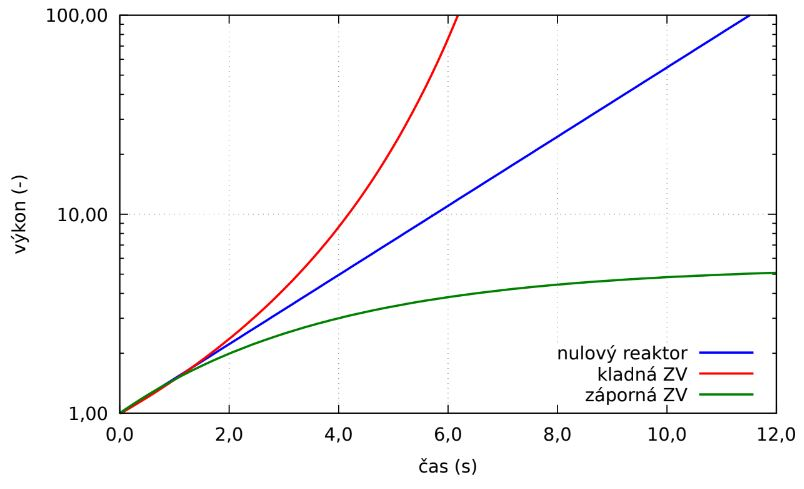
\includegraphics[width=0.7\textwidth]{img/ZV.JPG}
  \caption{Vliv ZV na zavedení kladné reaktivity.}
  \label{ZV}
\end{figure}

Graf dále ukazuje, že při velmi nízkých výkonech (nulový reaktor) všechny křivky splývají, jelikož se vliv ZV zatím neuplatňuje. Lze tedy říci, že každý reaktor se chová jako nulový a každý reaktor má ZV, pouze závisí, od jakého výkonu se začnou projevovat.\\

Dále je možné ZV rozlišit pomocí fyzikálních vlastností:

\begin{itemize}
  \item jaderné -- změnou teploty se mění mikroskopické účinné průřezy (Doppler), zároveň se může změnit Maxwell-Boltzmannovo rozdělení hustoty toku (maximum se posune do vyšších energií), což má za následek změnu reakčních rychlostí,
  \item hustotní -- změnou teploty se mění hustota jader a tím makroskopické účinné průřezy, nebo geometrické změny ovlivní Buckling.
\end{itemize}

\subsubsection{Doppler}

Dopplerovo rozšíření je kapitola sama o sobě. To se uplatňuje pouze v rezonancích, kde vlivem teplotní změny dochází k poklesu maxima a nárůstu šířky peaku tak, aby plocha pod peakem zůstala konstantní (vlivem teplotní změny atomy více kmitají, a proto se jakoby "rozmazávají"). Jelikož neutron ztrácí svoji energii po skocích, ne kontinuálně, při rozšíření základny rezonance vzniká "větší prostor", kam může neutron spadnout a dojít k záchytu.\\

Ve výsledku, Dopplerovo rozšíření vždy způsobuje zvyšování abrosbce, otázka je, jestli jde o radiační záchyt, nebo štěpení. Pro okolní materiály mimo palivo (moderátor, chladivo, konstrukce) vždy dochází k radiačnímu záchytu, jde tedy o zápornou ZV která vede k poklesu reaktivity.\\

U paliva záleží na konkrétním izotopickém složení a obohacení. Například pro U-238 je Doppler velmi významný, jelikož při zpomalování neutronu už ho neutron nemůže štěpit a dochází právě k radičnímu záchytu. Naopak u U-235 by sice došlo k nárůstu absorbce, ale tím i nárůstu štěpení. Je proto důležitý poměr obohacení. Na KIDu jsme si říkali, že při obohacení pod 35\% dojde vždy k převládnutí parazitní abrosrbce na U-238 a tedy k poklesu reaktivity. Pod touto hranicí jde tedy o zápornou ZV (tepelné reaktory), nad tuto hranici je třeba být opatrný, jelikož může vést ke kladné ZV (rychlé reaktory).

\subsubsection{Vodo-uranový poměr}

Tepelné jaderné reaktory potřebují k udržení štěpné řetězové reakce tepelné neutrony, které vznikají zpomalováním v moderátoru. Při změně teploty moderátoru dochází rovněž ke změně jeho hustoty a tím i ke změně makroskopických průřezů a reakčních rychlostí. Při změně teploty moderátoru tak nutně dochází ke změně moderačních vlastností a tím i ke změně reaktivity.\\

Aby bylo možné analyzovat, jak se změna hustoty moderátoru projeví na změně reaktivity, je třeba určit průběh závislosti reaktivity na hustotě moderátoru (\textbf{vodo-uranový poměr}), viz obrázek \ref{voda-uran}. Z toho lze rozlišit 2 typy moderátoru:

\begin{itemize}
  \item ideální moderátor (modrý) -- moderátor, na kterém nedochází k žádné parazitní absorbci,
  \item skutečný moderátor (červená).
\end{itemize}

\begin{figure}[H]
  \centering
  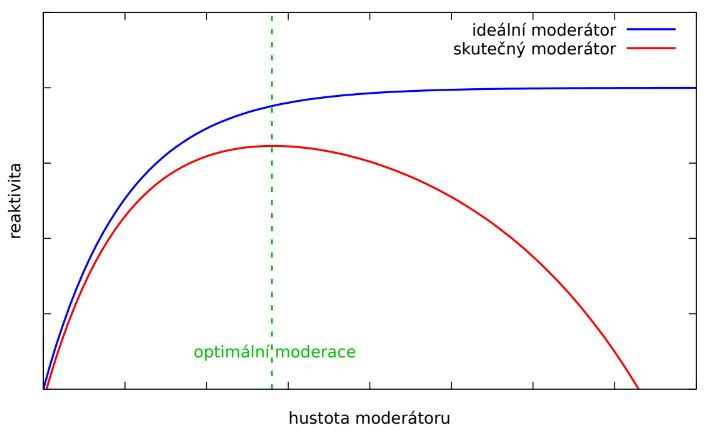
\includegraphics[width=0.7\textwidth]{img/voda-uran.JPG}
  \caption{Závislost reaktivity na hustotě moderátoru.}
  \label{voda-uran}
\end{figure}

Při přidávání ideálního moderátoru dochází pouze k větší termalizaci a žádné parazitní absorbci, proto reaktivita roste a ustaluje se na saturované hodnotě. Ve skutečnosti ale při přidávání moderátoru od jistého okamžiku dojde k převládnutí parazitní absorbce a reaktivita opět klesá. K maximu reaktivity pak dochází při tzv. \textbf{optimální moderaci}, část vlevo se poté nazývá \textbf{podmoderovaná} (méně moderátoru než je optimum) a část vpravo \textbf{přemoderovaná}. Tvar této křivky závisí na konkrétním moderátoru (zde je vidět např. výhoda těžké vody oproti lehké vodě, kdy na těžké dochází k absorbci výrazně méně).\\

Známe-li tyto grafy, je možné analyzovat, co se stane při změně teploty. Při zvyšování teploty dojde k poklesu hustoty moderátoru, což v řeči grafu \ref{voda-uran} znamená posun doleva. Pokud se budeme nacházet v podmoderované oblasti, dojde k poklesu reaktivity (ZV). Nicméně v přemoderované oblasti dojde k nárůstu (kladná ZV). Z hlediska bezpečnosti je proto důležité mít reaktor v podmoderované oblasti, což je možné ovlivnit: geometrií, obohacením, vyhořením, koncentrací boru apod. Zároveň může docházet k lokálnímu přemoderování (výzkumné reaktory), důležité je ale celkový charakter.

\subsection{Zpětnovazební koeficienty reaktivity}

\textbf{Zpětnovazební koeficienty} mohou být jakékoliv (teplotní, hustotní, výkonové), nicméně většinou je stejně vše ovlivněno právě teplotou (teplota ovlivní hustotu, změna výkonu ovlivní teplotu apod.), tudíž se dále zaměříme pouze na ty teplotní. Ty je možné určit dle vztahu:

\begin{equation}
  \boxed{
  a_i = \dfrac{\partial \rho}{\partial T_i}
  \label{zpetnovazebni_koeficient_definice}
  }
\end{equation}

A celkový vliv na reaktivitu jako:

\begin{equation}
  \boxed{
  \rho_{tot} = \sum_i \dfrac{1}{V_i} \int_{V_i} a_i(\bar{r}) \Delta T_i(\bar{r}) \Omega_i(\bar{r}) d\bar{r},
  \label{zpetnovazebni_koeficient_reaktivita}
  }
\end{equation}

kde:

\begin{itemize}
  \item $\Delta T_i$ -- představuje teplotní odchylku od i-té složky (teplotní rozdíl od kritického a aktuálního stavu),
  \item $\Omega_i$ představuje tzv. \textbf{normovanou váhovou funkci}, která opravuje fakt, že stejné teplotní změny mohou mít v jiných místech jiný vliv na reaktivitu. Skutečně jsou úměrné $\Phi^2$.
\end{itemize}

Při použití jednobodové kinetiky je možné zanedbat prostorovou závislost. Pokud se navíc zavede lineární model zpětné vazby, kdy budou koeficienty konstantní (normálně jsou závislé na teplotě), tak se výpočet zjednodušší:

\begin{equation}
  \boxed{
  \rho_{tot} = \sum_i a_i \Delta T_i (t).
  \label{zpetnovazebni_koeficient_reaktivita_1B}
  }
\end{equation}

\subsection{Přenosová funkce zpětné vazby}

Vliv zpětně vazby je možné vyjádřit i pomocí jednobodové kinetiky/dynamiky. Z linearizovaného modelu nulového reaktoru vyplývá (směr "doprava", tedy jak změna reaktivity vede na změnu četnosti):

$$ \dfrac{\Delta \tilde{N}(s)}{N_0} = \tilde{G_0}(s) \cdot \tilde{\rho}(s) = \tilde{G_0}(s) \cdot [ \tilde{\rho_\text{ex}}(s) + \tilde{\rho_\text{ZV}}(s) ], $$

kde $\tilde{\rho_\text{ex}}(s)$ značí vnesenou reaktivitu a $\tilde{\rho_\text{ZV}}(s)$ reaktivitu zpětné vazby. Zároveň je ale tato ZV reaktivita ovlivněna změnou četnosti, proto musí mít vlastní \textbf{přenosovou funkci zpětné vazby} $\tilde{W_\text{ZV}}(s)$, pro kterou platí\footnote{Tentokrát se přenosová funkce ZV definuje "obráceně", viz linearizovaný model v předešlé otázce. Tudíž pro $G_0$ platí, že změna reaktivity ovlivní četnost, ale tady platí, že změna četnosti ovlivní velikost ZV reaktivity.} (směr "doleva", tedy jak změna četnosti ovlivní reaktivitu, nicméně tentokrát pouze tu zpětnovazební):

$$ \tilde{\rho_\text{ZV}}(s) = \tilde{W_\text{ZV}}(s) \cdot \dfrac{\Delta \tilde{N}(s)}{N_0}. $$

Když se to všechno poskládá do sebe, tak je možné získat finální tvar spolu s tzv. \textbf{přenosovou funkcí reaktoru}\footnote{Tentokrát už nenulového.} $\tilde{G}(s)$ ve tvaru:

\begin{equation}
  \boxed{
    \dfrac{\Delta \tilde{N}(s)}{N_0} = \tilde{G}(s) \cdot \tilde{\rho}(s) = \dfrac{\tilde{G_0}(s)}{1 - \tilde{G_0}(s) \tilde{W_\text{ZV}}(s)} \cdot \tilde{\rho}(s).
  }
\end{equation}

Zbývá určit pouze tvar přenosové funkce zpětné vazby, čímž se získá tvar celkové přenosové funkce a vše se může řešit stejnými postupy, jako v případě kinetiky.\\

Zároveň se ještě hodí znát podmínku stability reaktoru, tedy situaci, jestli se výkon po nějaké době ustálí, nebo diferguje do nekonečna. Zde platí jednoduchý vztah:

\begin{equation}
  \boxed{
    \int_0^\infty  |G(t)| dt < \infty.
  }
\end{equation}

Zde platí, že nulový reaktor je vždy nestabilní. Stabilizuje se pouze až se zápornými ZV.

\subsection{Modely dynamiky reaktoru}

Analytické vyjádření zpětnovazební přenosové funkce je obtížné, často se musí něco zanedbat apod. Existuje několik modelů v závislosti na tom, co se mění (ve všech případech jde o linearizované modely):

\begin{itemize}
  \item Dvousložkový model -- mění se pouze teplota paliva a chladiva (tlakovodní a sodíkové reaktory):\\
  $$ \tilde{W_\text{ZV}}(s) = \dfrac{a_\text{fuel} (1 + s \: \tau_\text{cool}) + a_\text{cool} \: \Gamma}{k_\text{fuel} \: [(1 + s \: \tau_\text{cool})(1 + s \: \tau_\text{fuel}) - \Gamma]} $$
  \item Jednosložkový model -- pouze jedna teplota (molten salt):\\
  $$ \tilde{W_\text{ZV}}(s) = \dfrac{a_\text{power}}{1 + s \: \tau}. $$
  \item Adiabatický model -- rychlé změny, kdy se teplo nestačí odvézt:\\
  $$ \tilde{W_\text{ZV}}(s) = \dfrac{a_\text{fuel}}{s \: C_\text{fuel}}. $$
\end{itemize}

Ve všech případech: $a$ značí koeficient reaktivity, $C$ tepelnou kapacitu, $k$ součinitel prostupu tepla a konstanty $\tau$ a $\Gamma$ jsou jisté časové, resp. bezrozměrné konstanty, které pouze zjednodušují zápis a pro každý model se volí jinak. Více modelů a jejich odvození je v Bédových skriptech.


\section[Zpětné vazby]{Zpětné vazby v jaderném reaktoru, principy jejich působení a důsledky pro dynamiku jaderného reaktoru}

\textbf{Zpětná vazba} (ZV) = proces, díky kterému se změna výstupních parametrů ($P$, $\Phi$) může podílet na změnu vstupních parametrů.

\textbf{Dynamika reaktoru} = to samé co kinetika, pouze už uvažuje zapojení ZV.

Cílem dynamiky reaktorů je řešit ZV. Vlivem ZV se nám totiž reaktivita mění (teplota, tlak, roztažnost...). Vše je primárně ovlivněno teplotou, jelikož s rosroucí reaktivitou roste výkon a tím i teplota systému. Celkovou reaktivitu můžeme určit jako součet reaktivity dodané zvenčí (tyče, palivo, konfigurace) a reaktivity ve ZV.

\subsection{Zpětné vazby}

ZV mohou být obecně:

\begin{itemize}
  \item kladné -- odezva roste, nestabilita.
  \item záporné -- odezva klesá, čímž se reaktor může stabilizovat,
\end{itemize}

Pokud se do reaktoru zavede kladná reaktivita s vlivem kladné zpětné vazby, a zároveň není-li reaktivita potlačena (tyčemi apod.), může i tato malá změna vést k nekontrolovanému nárůstu výkonu (rychlejší než exponenciální). Naopak, projeví-li se záporná zpětná vazba, reaktor se po chvíli stabilizuje. A na jaké hodnotě? Tehdy, pokud se reaktivity vyrovnají (kladná vnesená reaktivita se vyrovná záporné reaktivitě vziklé vlivem ZV $\rightarrow$ Celkový efekt je na nule), což závisí na velikosti vnesené reaktivity a velikosti zpětnovazebních koeficientů. Záporné ZV pomáhají k řízení reaktoru, jelikož vždy působí proti počáteční změně a mají tendenci reaktor stabilizovat, viz graf \ref{ZV}.

\begin{figure}[H]
  \centering
  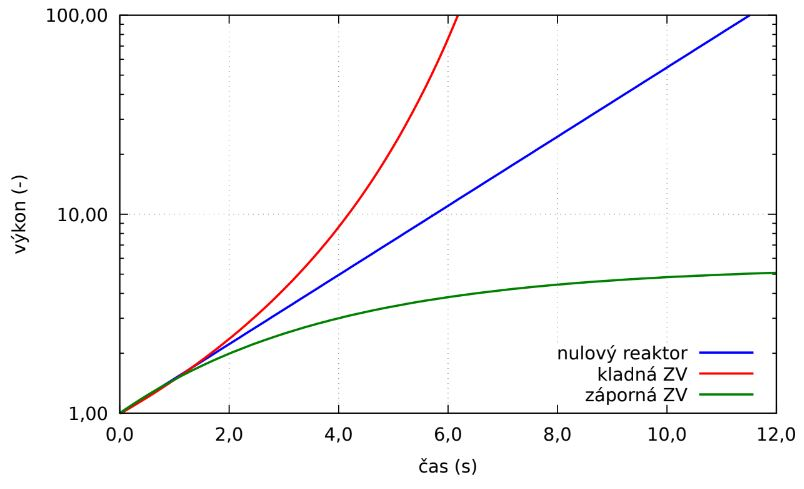
\includegraphics[width=0.7\textwidth]{img/ZV.JPG}
  \caption{Vliv ZV na zavedení kladné reaktivity.}
  \label{ZV}
\end{figure}

Graf dále ukazuje, že při velmi nízkých výkonech (nulový reaktor) všechny křivky splývají, jelikož se vliv ZV zatím neuplatňuje. Lze tedy říci, že každý reaktor se chová jako nulový a každý reaktor má ZV, pouze závisí, od jakého výkonu se začnou projevovat.

Dále je možné ZV rozlišit pomocí fyzikálních vlastností:

\begin{itemize}
  \item jaderné -- změnou teploty se mění mikroskopické účinné průřezy (Doppler), zároveň se může změnit Maxwell-Boltzmannovo rozdělení hustoty toku (maximum se posune do vyšších energií), což má za následek změnu reakčních rychlostí,
  \item hustotní -- změnou teploty se mění hustota jader a tím makroskopické účinné průřezy, nebo geometrické změny ovlivní Buckling.
\end{itemize}

\subsubsection{Doppler}

Dopplerovo rozšíření je kapitola sama o sobě. To se uplatňuje pouze v rezonancích, kde vlivem teplotní změny dochází k poklesu maxima a nárůstu šířky peaku tak, aby plocha pod peakem zůstala konstantní (vlivem teplotní změny atomy více kmitají, a proto se jakoby "rozmazávají"). Jelikož neutron ztrácí svoji energii po skocích, ne kontinuálně, při rozšíření základny rezonance vzniká "větší prostor", kam může neutron spadnout a dojít k záchytu.

Ve výsledku, Dopplerovo rozšíření vždy způsobuje zvyšování abrosbce, otázka je, jestli jde o radiační záchyt, nebo štěpení. Pro okolní materiály mimo palivo (moderátor, chladivo, konstrukce) vždy dochází k radiačnímu záchytu, jde tedy o zápornou ZV která vede k poklesu reaktivity.

U paliva záleží na konkrétním izotopickém složení a obohacení. Například pro U-238 je Doppler velmi významný, jelikož při zpomalování neutronu už ho neutron nemůže štěpit a dochází právě k radičnímu záchytu. Naopak u U-235 by sice došlo k nárůstu absorbce, ale tím i nárůstu štěpení. Je proto důležitý poměr obohacení. Na KIDu jsme si říkali, že při obohacení pod 35\% dojde vždy k převládnutí parazitní abrosrbce na U-238 a tedy k poklesu reaktivity. Pod touto hranicí jde tedy o zápornou ZV (tepelné reaktory), nad tuto hranici je třeba být opatrný, jelikož může vést ke kladné ZV (rychlé reaktory).

\subsubsection{Vodo-uranový poměr}

Tepelné jaderné reaktory potřebují k udržení štěpné řetězové reakce tepelné neutrony, které vznikají zpomalováním v moderátoru. Při změně teploty moderátoru dochází rovněž ke změně jeho hustoty a tím i ke změně makroskopických průřezů a reakčních rychlostí. Při změně teploty moderátoru tak nutně dochází ke změně moderačních vlastností a tím i ke změně reaktivity.

Aby bylo možné analyzovat, jak se změna hustoty moderátoru projeví na změně reaktivity, je třeba určit průběh závislosti reaktivity na hustotě moderátoru (\textbf{vodo-uranový poměr}), viz obrázek \ref{voda-uran}. Z toho lze rozlišit 2 typy moderátoru:

\begin{itemize}
  \item ideální moderátor (modrý) -- moderátor, na kterém nedochází k žádné parazitní absorbci,
  \item skutečný moderátor (červená).
\end{itemize}

\begin{figure}[H]
  \centering
  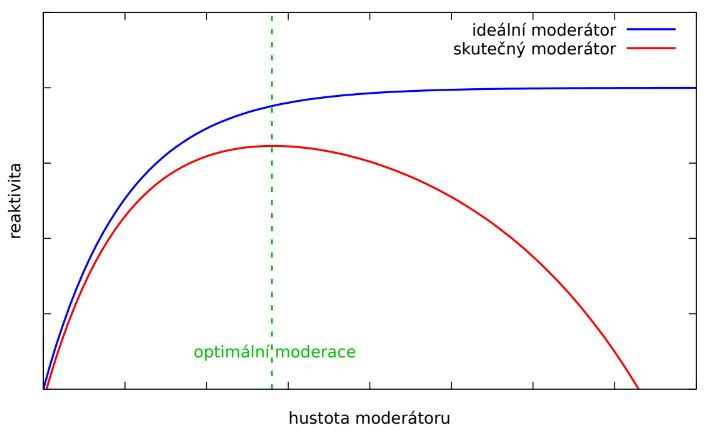
\includegraphics[width=0.7\textwidth]{img/voda-uran.JPG}
  \caption{Závislost reaktivity na hustotě moderátoru.}
  \label{voda-uran}
\end{figure}

Při přidávání ideálního moderátoru dochází pouze k větší termalizaci a žádné parazitní absorbci, proto reaktivita roste a ustaluje se na saturované hodnotě. Ve skutečnosti ale při přidávání moderátoru od jistého okamžiku dojde k převládnutí parazitní absorbce a reaktivita opět klesá. K maximu reaktivity pak dochází při tzv. \textbf{optimální moderaci}, část vlevo se poté nazývá \textbf{podmoderovaná} (méně moderátoru než je optimum) a část vpravo \textbf{přemoderovaná}. Tvar této křivky závisí na konkrétním moderátoru (zde je vidět např. výhoda těžké vody oproti lehké vodě, kdy na těžké dochází k absorbci výrazně méně).

Známe-li tyto grafy, je možné analyzovat, co se stane při změně teploty. Při zvyšování teploty dojde k poklesu hustoty moderátoru, což v řeči grafu \ref{voda-uran} znamená posun doleva. Pokud se budeme nacházet v podmoderované oblasti, dojde k poklesu reaktivity (ZV). Nicméně v přemoderované oblasti dojde k nárůstu (kladná ZV). Z hlediska bezpečnosti je proto důležité mít reaktor v podmoderované oblasti, což je možné ovlivnit: geometrií, obohacením, vyhořením, koncentrací boru apod. Zároveň může docházet k lokálnímu přemoderování (výzkumné reaktory), důležité je ale celkový charakter.

\subsubsection{Dutinový efekt}

V případě varných reaktorů může dojít k varu vody, čímž vnikne prostor s velkým objemem páry (tzv. dutina), což má za následek pokles moderace, ale zároveň opkles absorbce. Otázkou opět je, který efekt převládne.

Pro lehkovodní PWR reaktory platí, že mají záporný dutinový koeficient. Pokud zvýším průtok, zlepší se přenos tepla, dutiny se zmenší a výkonnaroste. To samé zvýší-li se tlak, tak se zvýší bod varu, dutiny se opět zmenší a výkon naroste. To je dobrý bezpečnostní efekt, při LOCE dojde ke snížení tlaku (klesá výkon) a ke snížení průtoku (klesá výkon).

Naopak RBMK má kladný dutinový koeficient, jelikož tam voda není zároveň moderátor. Lepší nestavět.

Pro PWR reaktory jde o nevýznamný efekt, tady dutiny nevznikají. Pokud ano, tak je něco špatně.

\subsection{Zpětnovazební koeficienty reaktivity}

\textbf{Zpětnovazební koeficienty} mohou být jakékoliv (teplotní, hustotní, výkonové), nicméně většinou je stejně vše ovlivněno právě teplotou (teplota ovlivní hustotu, změna výkonu ovlivní teplotu apod.), tudíž se dále zaměříme pouze na ty teplotní. Ty je možné určit dle vztahu:

\begin{equation}
  \boxed{
  a_i = \dfrac{\partial \rho}{\partial T_i}
  \label{zpetnovazebni_koeficient_definice}
  }
\end{equation}

A celkový vliv na reaktivitu jako:

\begin{equation}
  \boxed{
  \rho_{tot} = \sum_i \dfrac{1}{V_i} \int_{V_i} a_i(\bar{r}) \Delta T_i(\bar{r}) \Omega_i(\bar{r}) d\bar{r},
  \label{zpetnovazebni_koeficient_reaktivita}
  }
\end{equation}

kde:

\begin{itemize}
  \item $\Delta T_i$ -- představuje teplotní odchylku od i-té složky (teplotní rozdíl od kritického a aktuálního stavu),
  \item $\Omega_i$ představuje tzv. \textbf{normovanou váhovou funkci}, která opravuje fakt, že stejné teplotní změny mohou mít v jiných místech jiný vliv na reaktivitu. Skutečně jsou úměrné $\Phi^2$.
\end{itemize}

Při použití jednobodové kinetiky je možné zanedbat prostorovou závislost. Pokud se navíc zavede lineární model zpětné vazby, kdy budou koeficienty konstantní (normálně jsou závislé na teplotě), tak se výpočet zjednodušší:

\begin{equation}
  \boxed{
  \rho_{tot} = \sum_i a_i \Delta T_i (t).
  \label{zpetnovazebni_koeficient_reaktivita_1B}
  }
\end{equation}

\subsection{Přenosová funkce zpětné vazby}

Vliv zpětně vazby je možné vyjádřit i pomocí jednobodové kinetiky/dynamiky. Z linearizovaného modelu nulového reaktoru vyplývá (směr "doprava", tedy jak změna reaktivity vede na změnu četnosti):

$$ \dfrac{\Delta \tilde{N}(s)}{N_0} = \tilde{G_0}(s) \cdot \tilde{\rho}(s) = \tilde{G_0}(s) \cdot [ \tilde{\rho_\text{ex}}(s) + \tilde{\rho_\text{ZV}}(s) ], $$

kde $\tilde{\rho_\text{ex}}(s)$ značí vnesenou reaktivitu a $\tilde{\rho_\text{ZV}}(s)$ reaktivitu zpětné vazby. Zároveň je ale tato ZV reaktivita ovlivněna změnou četnosti, proto musí mít vlastní \textbf{přenosovou funkci zpětné vazby} $\tilde{W_\text{ZV}}(s)$, pro kterou platí\footnote{Tentokrát se přenosová funkce ZV definuje "obráceně", viz linearizovaný model v předešlé otázce. Tudíž pro $G_0$ platí, že změna reaktivity ovlivní četnost, ale tady platí, že změna četnosti ovlivní velikost ZV reaktivity.} (směr "doleva", tedy jak změna četnosti ovlivní reaktivitu, nicméně tentokrát pouze tu zpětnovazební):

$$ \tilde{\rho_\text{ZV}}(s) = \tilde{W_\text{ZV}}(s) \cdot \dfrac{\Delta \tilde{N}(s)}{N_0}. $$

Když se to všechno poskládá do sebe, tak je možné získat finální tvar spolu s tzv. \textbf{přenosovou funkcí reaktoru}\footnote{Tentokrát už nenulového.} $\tilde{G}(s)$ ve tvaru:

\begin{equation}
  \boxed{
    \dfrac{\Delta \tilde{N}(s)}{N_0} = \tilde{G}(s) \cdot \tilde{\rho}(s) = \dfrac{\tilde{G_0}(s)}{1 - \tilde{G_0}(s) \tilde{W_\text{ZV}}(s)} \cdot \tilde{\rho}(s).
  }
\end{equation}

Zbývá určit pouze tvar přenosové funkce zpětné vazby, čímž se získá tvar celkové přenosové funkce a vše se může řešit stejnými postupy, jako v případě kinetiky.

Zároveň se ještě hodí znát podmínku stability reaktoru, tedy situaci, jestli se výkon po nějaké době ustálí, nebo diferguje do nekonečna. Zde platí jednoduchý vztah:

\begin{equation}
  \boxed{
    \int_0^\infty  |G(t)| dt < \infty.
  }
\end{equation}

Zde platí, že nulový reaktor je vždy nestabilní. Stabilizuje se pouze až se zápornými ZV.

\subsection{Modely dynamiky reaktoru}

Analytické vyjádření zpětnovazební přenosové funkce je obtížné, často se musí něco zanedbat apod. Existuje několik modelů v závislosti na tom, co se mění (ve všech případech jde o linearizované modely):

\begin{itemize}
  \item Dvousložkový model -- mění se pouze teplota paliva a chladiva (tlakovodní a sodíkové reaktory):\\
  $$ \tilde{W_\text{ZV}}(s) = \dfrac{a_\text{fuel} (1 + s \: \tau_\text{cool}) + a_\text{cool} \: \Gamma}{k_\text{fuel} \: [(1 + s \: \tau_\text{cool})(1 + s \: \tau_\text{fuel}) - \Gamma]} $$
  \item Jednosložkový model -- pouze jedna teplota (molten salt):\\
  $$ \tilde{W_\text{ZV}}(s) = \dfrac{a_\text{power}}{1 + s \: \tau}. $$
  \item Adiabatický model -- rychlé změny, kdy se teplo nestačí odvézt:\\
  $$ \tilde{W_\text{ZV}}(s) = \dfrac{a_\text{fuel}}{s \: C_\text{fuel}}. $$
\end{itemize}

Ve všech případech: $a$ značí koeficient reaktivity, $C$ tepelnou kapacitu, $k$ součinitel prostupu tepla a konstanty $\tau$ a $\Gamma$ jsou jisté časové, resp. bezrozměrné konstanty, které pouze zjednodušují zápis a pro každý model se volí jinak. Více modelů a jejich odvození je v Bédových skriptech.



\end{document}
